%% Copyright 2007-2018 Elsevier Ltd
%% This file is part of the 'Elsarticle Bundle'.

%% Use the option review to obtain double line spacing
%% Use the options 1p,twocolumn; 3p; 3p,twocolumn; 5p; or 5p,twocolumn
\documentclass[preprint,1p, 10pt,authoryear]{elsarticle}
%%\documentclass[final,1p,times,authoryear]{elsarticle}
%\documentclass[final,1p,times,twocolumn,authoryear]{elsarticle}
 %%\documentclass[preprint,3p,times,authoryear]{elsarticle}
%% \documentclass[final,3p,times,twocolumn,authoryear]{elsarticle}
%% \documentclass[final,5p,times,authoryear]{elsarticle}
%% \documentclass[final,5p,times,twocolumn,authoryear]{elsarticle}

\usepackage{multicol}
\usepackage{graphicx}
\graphicspath{{./Graphic/}}
\usepackage{array}
\usepackage{amssymb} % various useful mathematical symbols
\usepackage{gensymb} % for `degree' sign
\usepackage{amsthm}  % extended theorem environments
\usepackage{lineno}   % for line numbers
\usepackage{amsmath} % for math operations
\usepackage{mathtools} % for math operations
\usepackage{tabularx} % for adjustable table width
\usepackage[hidelinks]{hyperref}  % for hyperlinks
\usepackage{amsmath}
\newtheorem{property}{Property}[section]
\usepackage{soul}
\usepackage{xcolor}
\usepackage{epsfig}
\usepackage{amssymb}  % various useful mathematical symbols
\usepackage{tabularx}
\usepackage{multirow} 
\usepackage{colortbl}
\usepackage{tablefootnote}
\usepackage{footnote}   
\usepackage{setspace}
\usepackage{rotating}
\usepackage{adjustbox}
\usepackage{blindtext}
\usepackage[printwatermark]{xwatermark}
\usepackage{xcolor}
\usepackage{graphicx}
\usepackage{lipsum}



\journal{Journal of Geophysical Research: Solid Earth}
\begin{document}


\begin{frontmatter}



\title{Modeling precursory laboratory seismicity using a wear-based rate- and state-dependent friction model}

 \author[1]{P. A. Selvadurai \corref{cor1}}
 \ead{paul.selvadurai@sed.ethz.ch}
\author[2]{P. Galvez}
\author[2]{P. M. Mai}
\author[3]{S. D. Glaser} 
\author[2]{D. B. Peter}
\author[1]{S. Wiemer} 



\cortext[cor1]{Corresponding author, Post-Doctoral fellow}
\address[1]{Swiss Seismological Service, ETH Zurich, Zurich, Switzerland}
\address[2]{King Abdullah University of Science and Technology, Thuwal, Saudi Arabia}
\address[3]{Civil and Environmental Engineering, University of California, Berkeley, California, USA}

%\begin{keypoints}
%\item Rate and state friction (RSF) models were developed from roughness measurements of a friction experiment that displayed properties of wear
%\item Simulations showed that smooth sections nucleated events that ruptured and were arrested by local roughened sections representing barriers
%\item Source properties of the RSF ruptures were compared to independently measured kinematic estimates from a concerted study for the first time
%\end{keypoints}


\begin{abstract}
We develop a rate- and state-dependent friction (RSF) model using the quasi-dynamic earthquake rupture simulator QDYN to investigate a compendium of recent experiments  performed on a fault analog. A fault was sheared until macroscopic stick-slip frictional failure occurred. Before the macro-failure small precursory seismicity nucleated from regions that also experienced aseismic slow slip. In some cases these precursory events did not cascade-up into gross fault rupture and arrested locally. The RSF model aims at understanding why spontaneous shear events occurred in the same region that also supported slow aseismic slip.  

A key ingredient needed for this observation is heterogeneity and our model infers local variation in frictional parameters from the roughness.  The surface was characterized \textit{a posteriori} and displayed clear evidence of wear in the form of a bimodal Gaussian distribution of surface height. This unique superposition of smooth and rough Gaussian surface heights was used to impose the spatial heterogeneity in the critical slip distance $D_{c}$ , which was equivalent to variations in the fracture energy $G^{'}$.  The model found that local seismicity nucleated on the ``smooth/polished'' sections, while the larger ``rough'' section hosted aseismic slip. As the level of heterogeneity between smooth and rough sections increased, the model transitioned from a predominantly stick-slip dominant to creep-like behavior.  The simulations produced a dominant asperity, which appeared to control aspects of rupture nucleation. At low levels of heterogeneity, the dominant asperity failed in a regular manner but could also `cascade up'  and produce a fault-wide event. At high-levels of heterogeneity, ruptures on the dominant asperity remained constrained and exhibited repeater-like behavior. Seismic source properties: average slip $\delta$, seismic moment $M_{0}$, stress drop $\Delta \tau$ and fracture energy $G^{'}$, were determined for each event and agreed with separate kinematic estimates made independently from the measured ground motions produced by elastodynamic stress waves. Our numerical calculations provide insight into seismicity produced from frictional heterogeneity associated with fault mirrors in laboratory.

\end{abstract}
%\section*{Plain Language Summary}
%Recent seismic observations show that faults experience a range of slip patterns spanning many scales in both space and time. Understanding how slip accumulates on complex fault systems can lead to a better understanding of regions that are more prone and susceptible to large events.

%We developed a friction model that we used to study results from a scaled frictional fault in the laboratory. This fault also showed complex slip behavior. We notice that scaled versions of earthquakes occurred in larger regions that were also slipping more slowly. This behavior has also been observed in nature but we are not certain as to why exactly. We linked this behavior to a mathematical model that describes friction on faults. To add complexity, we used the experimental roughness measured along the interface, which might explain the complicated slip patterns. Using the roughness, we found that the model produced earthquakes patterns and general behaviors that matched many experimental measurements taken independently. We found that complexity formed by fault roughness can produce a wide range of slip behaviors that are also observed in natural systems at many scales. Understanding how roughness evolves over a fault's lifetime will be important for moving forward earthquake science.  


\begin{keyword}
Earthquake nucleation, foreshocks, laboratory experiments, rate and state friction, wear, fault mirrors, asperities, seismic source properties
\end{keyword}

\end{frontmatter}
\doublespacing
\linenumbers



\section{Introduction}
\label{int}
Growing amounts of seismologic observations capture ever larger diversity in slip behavior along natural faults. Observations, such as, spatio-temporally variations in seismicity rates \citep{Tormann2014, Tormann2015, Gulia2016,Gulia2019}, the presence of repeaters in aseismically creeping fault sections \citep[e.g.][]{Nadeau1994, Nadeau1999, Shirzaei2013, Uchida2019}, variations of slow slip distribution over large scales inferred from geodetic measurement  \citep[e.g.][]{Brodsky2014, Ruiz2014, Socquet2017}, the earthquake potential on sections prone to large ruptures \citep{Buergmann2000,Buergmann2004}, the observed variability in spatio-temporal slip patterns during rapid rupture \citep[e.g.][]{Mai2002, Tinti2005, Dreger2007, Galvez2016, Mai2018} suggest that coupling of faults and its ability to resist frictional breakdown is heterogeneous. 

Heterogeneity in frictional properties is also necessary to explain the observation that, in certain cases, precursory seismicity has been observed in regions that also supports the steady growth of a preslip region \citep{Kato2012, Kato2016, Obara2016, Ruiz2014, Bouchon2013,Buergmann2004}. Preslip is a slow accumulation of fault slip in a region that grows outwards to a critical size where it becomes unstable and the mainshock ensues \citep{Ohnaka1992, Ben-Zion2009}. This portion of the seismogenic cycle is known as the nucleation phase. This behavior has been identified from the onset of the mainshock's seismogram \citep{Iio1995, Ellsworth1995, Beroza1996} and recent improvements in geodetic measurements have been able to lower the detectable threshold and identify the nucleation phase over long time scales (months to years) and length scales (kms) \citep[e.g.,][]{Roeloffs2006,Ruiz2014, Socquet2017}.  In certain cases, a specific type of precursory seismicity known as foreshocks, have been observed prior to the mainshock \citep[e.g.,][]{Dodge1995, Dodge1996, Bouchon2011}. While it is unclear if all mainshocks are preceded by foreshocks \citep{Brodsky2014, Mignan2014, Seif2018} they are currently only detectable in retrospective analysis. Due to the forecasting potential offered by foreshocks -- how and why they occur and how do they affect the timing and severity of the impending mainshock -- they have become an important phenomena to study.

The study of the spatio-temporal growth of a preslip region  and its transition from slow (quasi-static) to fast (dynamic) slip has been well documented in laboratory experiments \citep{Dieterich1978,Okubo1984, Ohnaka1999, Nielsen2010, Latour2013, Fukuyama2018, Zhuo2018, Ke2018, Buijze2020}. More recently, along with measuring the spatio-temporal evolution of slow preslip region, acoustic emission sensors were deployed that detected localized, high-frequency and impulsive events that spontaneously emanate from sections of the fault that also hosted the preslip front \citep{Ma2002, McLaskey2013, Selvadurai2015, Zhuo2018a}.  Analysis of these localized events using seismological models found the moment released with respect to their geometry scaled with earthquakes in nature \citep{McLaskey2014, Selvadurai2019}. This similarity has sparked more interest to understand the implications laboratory foreshocks have on the growth and stability of the preslip region and the influence of foreshocks themselves on the size and timing of the larger mainshock \citep{McLaskey2019}.  A major question is when does a foreshocks `cascade-up' into the the mainshock? Studies of the initial onset of a seismic rupture via seismograms, appear to indicate that asperities exist at many spatial scales, and that the triggering of cascading-style failure mechanism might stem from the failure of a smaller section of the fault \citep{Okuda2018, Ide2019}. This type of hierarchical breakdown may be indicating the possible existence of a hierarchical plate interface structure \citep{Ide2005, Aochi2014, Aochi2017}.  Foreshocks might be local failures of these asperities that do not fully `cascade-up' but do posses this runaway potential if conditions are conducive. 

Conditions that controls the occurrence of foreshocks (or other types of precursory seismicity) during the nucleation phase at even laboratory scales is not entirely clear. In the previously highlighted laboratory foreshocks studies \citep{McLaskey2013, Selvadurai2015}, the fault behavior was dictated by a dry and gouge-free fault environment.  In this cases, the heterogeneity is believed to occur because of the geometric interaction between the two rough surfaces that give rise to contact asperities with locally high normal stresses.  The contact heterogeneity was confirmed by \citet{Selvadurai2017} with measurement of spatially variable normal stress determined from a pressure sensitive film place along the rough-rough interface but this has also been widely investigated in the field of statistical contact mechanics \citep[e.g.][]{Greenwood1966,Johnson1985, Persson2006}. 

Mechanisms as why foreshocks spontaneously occur in sections of accumulating slip were examined.  \citet{Selvadurai2017} proposed that the localized precursory events occurred on asperities that exhibit higher levels of normal stress, thus locally decreasing its critical nucleation length scale (defined later in Section \ref{Theory}). If the asperity was geometrically large enough it could facilitate the spontaneous localization of dynamic failure in the presence of preslip. This hypothesis was later presented by \citet{McLaskey2019}. Another mechanism proposed by \citet{McLaskey2013} was that the increased stressing rate around the local geometric interference between surfaces might contribute to higher shear stresses resulting in the dynamic failure of these contact asperities.  

An equally interesting counterpoint is why does the foreshocks arrest? What type/level of frictional heterogeneity is necessary to arrest the rupture that should, on a homogeneous interface, continue to rupture the entire frictional interface? From the study of dynamic rupture propagation, after spontaneous initiation of dynamic rupture, the slip fronts begins to expand in a crack-like manner, accelerating outwards to a critical velocity, whereby it may transition to a pulse-like dynamic rupture \citep{Heaton1990, Meier2016}. Experiments and numerical investigations into the causes for complex rapid rupture nucleation and arrest in the laboratory are highly dependent on the stress states on the fault ahead of the rupture \citep{Rubinstein2004, Rubinstein2006, Ben-David2010,Svetlizky2014,Fineberg2015, Maegawa2010, Tromborg2011, Kammer2012, Kammer2015} and appear to control even slower quasi-static ruptures \citep{Selvadurai2017a}. The study of why/how laboratory ruptures arrest in these studies are performed at larger scales than the high-frequency foreshocks measured with AE sensors. For this reason, it becomes difficult to study the interaction of the foreshock/nucleation region which requires, in the laboratory, a broadband temporal and spatial understanding of slip: from frequencies ranging from DC to $\sim$ 1.5 MHz and length scales ranging from tens of microns to meters. 

In this study, we aim to understand mechanisms for localized fast ruptures embedded within a slow rupture were asperities are formed from geometric mismatch of the two rough surfaces. We develop a numerical rate- and state-friction (RSF) model \citep{Dieterich1979,Ampuero2008, Rubin2005} that is used to explain a compendium of laboratory data from a specific direct shear friction experiment performed on a fault analog. The observations follow the recent publications and the reader should consult these studies for the experimental details. These studies examine the same experiment, which highlight:

\begin{enumerate}
\item \textbf{\citet{Selvadurai2015}: } A nucleation phase where a slow preslip front was observed prior to onset of a system wide stick-slip instabilities. Within this preslip region, localized foreshocks were observed;
\item \textbf{\citet{Selvadurai2017}:} Characteristics of the roughness and quantitative analysis of the contact stresses on the asperities were documented;
\item \textbf{\citet{Selvadurai2019}: }Seismic source properties of the localized foreshocks events that occurred in the preslip nucleation region were quantified using kinematic source models..
\end{enumerate}

\subsection{Summarized Experiment}
\label{GeneralExp}
A schematic diagram of the direct shear friction apparatus is shown in Figure \ref{fig1}(a). We refer to this scale as the macrosopic scale for the discussion. Experiments consisted of loading a long slender PMMA slider (12.7 mm x 406 mm x 80 mm) onto a larger PMMA base plate (610 mm x 305 mm x 51 mm). The interacting faces of the PMMA slider block and base plate were first sandblasted. During an experiment, the fault was maintained under constant normal load $F_{n}$.  The top slider was driven at a constant macroscopic loading rate $V_{LP}$ and an in-line shear load cell was used to measure the bulk frictional resistance $F_{S}$ along the fault (see Figure \ref{fig1}(b)).   
  
\begin{figure}
 	\centering
 	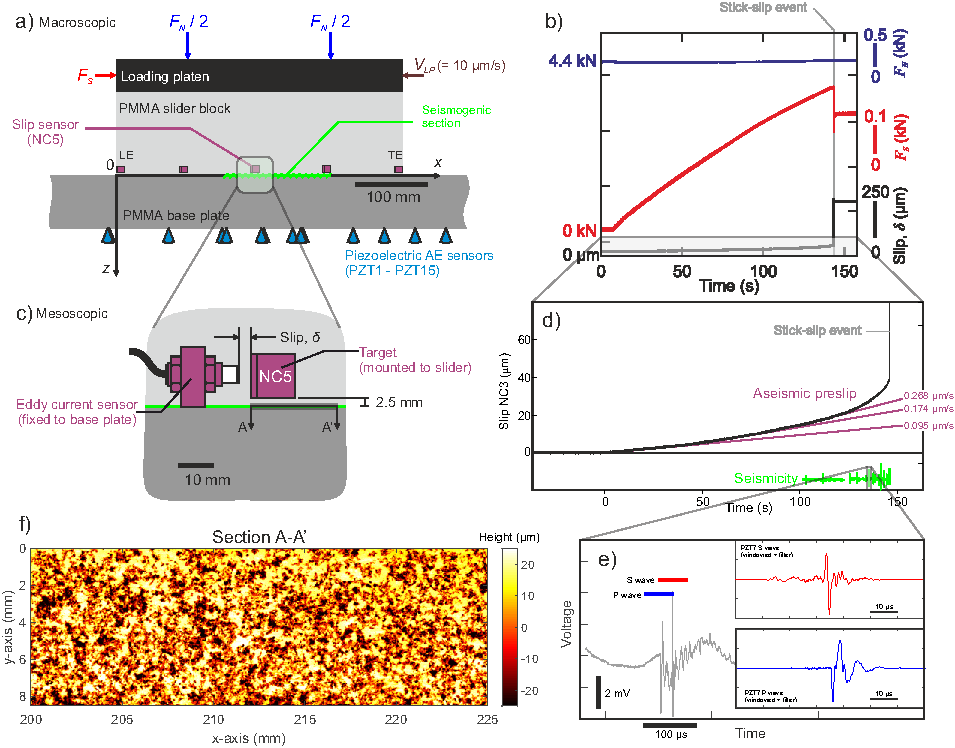
\includegraphics{FIG1_revised.pdf} 
 	\caption{ \textbf{(a)} Schematic details of the direct shear friction apparatus. General loading conditions and sensor placements are shown. For more technical details please consult the literature \citep{Selvadurai2015, Selvadurai2015a}. \textbf{(b)} Typical result demonstrating the bulk frictional evolution in terms of shear slip and shear force leading up to failure. \textbf{(c)} Schematic details of the non-contact eddy current sensor placement at the mesoscopic scale. \textbf{(d)} Detailed slip measurement during the experiment shown in (b).  Mesoscopic slow aseismic slip was observed leading up to macroscopic stick-slip failure.  Lines of constant slip velocity are shown for reference.  Seismicity (green) is represented schematically to show the presence of local fast slip as the accelerated aseismic slip was observed. \textbf{(e)}  An example of precursory seismicity recorded using PZT7.  Seismicity showed clear P and S wave arrivals. More detailed source analysis has been performed by \citet{Selvadurai2019}. \textbf{(f)} Surface roughness measurement taken \textit{a posteriori} using the longer length scale optical profilometer (Nanovea P50).  The region on the fault associated with this scan is shown by the cross-section A-A’ in (c).}
 	\label{fig1}
 \end{figure}
 In Figure \ref{fig1}(b) the slip evolution (black line) for the stick-slip event as measured by the non-contact eddy current sensor (NC5) is shown.  Figure \ref{fig1}(c) depicts a schematic representation of the eddy current sensor (mounted to the base plate) and the wing target attached to the slider block $\sim$ 2.5 mm on above the interface.  The inductive eddy current sensors measured slip $\delta$ in the $x$-direction. We refer to this scale as the mesosopic scale for the discussion.
 
During a stick-slip cycle the slow and smooth accumulation of aseismic as detailed in Figure \ref{fig1}(d). We show lines of constant slip rate (magenta), which are superimposed over the slip evolution curve.  The fault displayed an acceleration of aseismic slip leading up to the stick-slip event. This type of observation is fairly common in the laboratory friction experiments. However, we also observe pronounced impulsive events detected using the array of absolutely calibrated piezoelectric transducers (PZT) that measure high-frequency vibrations (100kHz to 1500 kHz) produced by stress waves. Seismicity is shown schematically (green) since the time scales between the slow slip and this impulsive source was $\sim$ 6 orders of magnitude different.  Figure \ref{fig1}(e) shows isolated P and S waves from a typical impulsive source measured by PZT7  \citep{Selvadurai2019}.
 
As mentioned before, our friction model requires spatial heterogeneity to explain the observations of synchronous and concomitant slow (Figure \ref{fig1}(d)) and fast rupture (Figure \ref{fig1}(e)). We base spatial heterogeneity in our RSF model on the experimental \textit{a posteriori} measurement of surface roughness. Figure \ref{fig1}(f) shows the optical scan of surface roughness on the top slider blocks surface through the cross-section A-A' in Figure \ref{fig1}(c).  The scans were taken below the non-contact sensor NC5 as shown.

\subsection{Surface Roughness Analysis}
\label{SRA}
We briefly describe certain methods used to quantify surface roughness in the fields of contact mechanics, tribology and geophysics that we will then use to characterize the interface shown in Figure \ref{fig1}(f). We deploy a measure of average roughness known as the root mean square:
\begin{equation}
h_{rms} = \sqrt{\left(\frac{1}{N} \right) \sum^{N}_{i=1} h_{i}^{2}} ,
\label{eq99}
\end{equation}
\noindent where $N$ is the total number of measurement points and $h_{i}$ is the individual surface height. To estimate statistical properties of surface heights we also employ the probability density functions (PDFs) of the surface height $h$ defined by a Gaussian distribution, which is given as follows:
\begin{equation}
\phi(h) = \left( 2\pi \sigma^{*} \right) exp\left[ \frac{\left(h - \mu^{*}\right)^{2}} { 2\sigma^{*2}}  \right],
\label{eq1}
\end{equation} 
\noindent where $\mu^{*}$ is the arithmetic mean and $\sigma^{*}$ is the standard deviation. Building on equation \eqref{eq1} we can also describe the PDF for a bimodal Gaussian mixture model as 
\begin{equation}
\Phi(h) = p\cdot \phi_{1}(h)+\left(1-p\right)\cdot \phi_{2}(h),
\label{eq2}
\end{equation}
\noindent where $p$ is the mixture ratio between the two Gaussian distribution functions $\phi_{1}$ and $\phi_{2}$, each with their individual means and standard deviations. When fitting \eqref{eq1} and \eqref{eq2} to the experimental measurements we employ a maximum likelihood estimation (MLE) of the means, standard deviations and mixture ratio. 

Finally, we also estimate surface properties using power spectral density (PSD), i.e.  the square of the modulus of the normalized Fourier transform, of a self-affine surface profile following 
\begin{equation}
P(k) \propto k^{-(1+2H)},
\label{eq999}
\end{equation}
\noindent where $k$ is the wavenumber and $H$ is the self-affine scaling exponent or Hurst exponent \citep{Power1991, Schmittbuhl1995, Candela2009}. The wavenumber $k = 1/\lambda$ where $\lambda$ is wavelength. By plotting equation \eqref{eq999} we can estimate $H$ using linear regression of log-log slope of the relationship between the PSD and wavenumber $\beta =-(1+2H)$.  

\subsection{Evidence of fault wear}
\label{SurfaceWear}
The facilities and measurement techniques are discussed in detail by \citet{Selvadurai2017}.  Figure \ref{fig2}(a) shows estimates of surface roughness using the root mean square (16. 7 $\mu$m using equation \eqref{eq99}), Gaussian (equation \eqref{eq1}) and bimodal Gaussian (equation \eqref{eq2}) distributions for the surface shown in Figure \ref{fig1}(f). The values of the means ($\mu^{*}$), standard deviations ($\sigma^{*}$) and mixture ratio ($p$) are shown for the modal (magenta) and bimodal (cyan) models are given in the figure with units of $\mu$m.  We see clearly that the shape of the distribution is more accurately characterized by the bimodal Gaussian distribution.  Evolution of roughness from Gaussian to bimodal Gaussian can be a quantified using the polish-rate decay (wear decay or \textit{Borucki} wear) function \citep{Borucki2002, Borucki2004, Ciavarella2016}. This type of distribution has been well-documented in the field of tribology and is used to characterize wear of the interface. As the surface wears from a Gaussian to bimodal Gaussian it reaches a steady state roughness.  A lapping procedure, described in \citet{Selvadurai2015}, detailed that $\sim$ 36.1 mm slip was needed before any type of foreshock/nucleation activity was observed and this is why we have considered the bimodal Gaussian distribution of roughness an important measurement in the development of our RSF model.  From the metrics, we see that wear has produced a smoother surface (i.e.  the `tail' in the PDF), and this polished surface exists within an encompassing rougher surface.     

\begin{figure}
	\centering
	\includegraphics{FIG2_revised.pdf} 
	\caption{\textbf{(a)} Surface height probability density function for the surface shown in Figure \ref{fig1}(f). Values of three surface roughness models are shown for the root mean square (black), Gaussian (magenta) and bimodal Gaussian (cyan) -- the values are given in $\mu$m. \textbf{(b)} Estimate of the Hurst exponent from the same surface are estimated from the power spectral density (PSD) described by equation \eqref{eq999} along the all transects in the $x-$direction (gray lines). The mean PSD for this surface is shown in black and Hurst exponent $H$ = 0.43 (red line). \textbf{(c)} Image of the worn PMMA fault surface from \citep{Selvadurai2015b} shows dark, smooth spots that are indicative of worn sections of the PMMA slider block. \textbf{(d)} Post-processing highlights the darker smooth sections. The inset image shows the spatial complexity of the smooth region. \textbf{(e)} Exposed outcrop with a mirror surface on a dolostone fault located along the Dead Sea Transform (image adapted from \citet{Goldberg2016}).  \textbf{(f)} Exposed outcrop with striated, glossy surface of the Corona Heights Fault (USA) (courtesy of J. E. Samuelson, taken from \citet{Verberne2019}).}
	\label{fig2}
\end{figure}
Figure \ref{fig2}(b) shows the results for estimating the Hurst exponent using the power spectral density estimates from the surface roughness transects in the $x-$direction. The average PSD was used to estimate a Hurst exponent $H$ = 0.43 between the wavenumbers of 1 mm $^{-1}$  $<k<$  50 mm $^{-1}$ from equation \eqref{eq999}. We note that any deviations of the values presented here from those in \citet{Selvadurai2017} are due to the more accurate cropping of the measurement region shown in Figure \ref{fig1}(f). 

Figure \ref{fig2}(c) shows a raw photograph of the surface from the seismogenic section of the fault (taken from \citet{Selvadurai2015b}). The image shows polished spots that had ``mirror-like'' finish that was responsible for the tail in the PDF of the surface roughness. From \citet{Selvadurai2017}, the polished surface `mirrors' were 188 times smoother than the overall RMS roughness for this the full region ($h_{RMS}$ = 16. 7 $\mu$m). Figure \ref{fig2}(d) highlights the darker regions by converting the raw image from RGB to light intensity between the range of 0 $< I <$ 0.35 \citep{Gonzales2004}. The inset image shows the complexity associated with the polished section. \citet[ch. 6, ][]{Selvadurai2015b} also shows images of a fresh (unworn) surface and these mirrors were not present.

The presence of FMs observed on natural outcrops have sparked interest form the geophysical community \citep{Fondriest2013,Kirkpatrick2013, Siman-Tov2013}.  The laboratory has been crucial in understanding the mechanism surrounding the formation of FMs and debate of whether the presence of a fault mirror can be used as an indicator for seismic slip \citep{Fondriest2013,Siman-Tov2013,Pozzi2018}, but they have also been reproduced in during slow slip \citep{Tisato2012,Siman-Tov2015}, in high-temperature environments \citep{Pluymakers2017} and observed along glacial boundaries \citep{Siman-Tov2017}. Figures \ref{fig2}(e) and (f) show two fault mirrors on the Dead Sea Transform and the Corona Heights Fault (USA) that formed at different scales, respectively.  \citet{Goldberg2016} believes that these FMs can potentially promote seismicity and also are believed to be more prevalent and can even occur at lower slip-rates than previously though \citep{Verberne2019}.  While there are differences between the mechanisms controlling how surfaces polish and FMs develop on rock-rock interfaces in hydro-thermal environments controlling and their development on a plastic PMMA surface \citep{Bouissou1998}, we are  more interested in how the initial conditions of how a ``smoother surface embedded in a rougher fault'' affects the frictional behavior using a RSF model. 

\section{Rate- and state-dependent (RSF) friction model}
\subsection{Theory}
\label{Theory}
RSF constitutive friction law is phenomenological and derived from laboratory experiments \citep{Dieterich1979, Ruina1983}.  The model describes the behavior of a faults resistance to sliding in terms of the shear stress $\tau$ as a function of the slip rate $V$ and a state variable $\theta$. This is given as:

\begin{equation}
\label{eq5}
\tau \left( V,\theta \right) = \sigma \left[\mu + a \ln\frac{V}{V^{*}} + b \ln\frac{V^{*}\theta}{D_{c}}\right],
\end{equation}   

\noindent where $\sigma$ is the effective normal stress, $\mu$ is the reference steady-state friction coefficient at an arbitrary reference slip rate $V^{*}$, $D_{c}$ is the characteristic slip distance and, $a$ and $b$ are constitutive parameters describing the direct and evolution effects, respectively.  The state parameter in our study is referred to as the so-called ``slip law’’ and is adopted due to its ability to model recent laboratory studies \citep{Bhattacharya2015, Kaneko2011, Kaneko2016}:

\begin{equation}
\label{eq6}
\dot{\theta} = - \frac{V\theta}{D_{c}}\ln\frac{V\theta}{D_{c}},
\end{equation}   

\noindent where friction at steady state ($\dot{\theta} $ = 0) is given as

\begin{equation}
\label{eq7}
\tau_{ss} \left( V \right) = \sigma \left[\mu + \left(a - b \right)\ln\frac{V}{V^{*}}\right].
\end{equation}   

\noindent From equation \eqref{eq7} we see that constitutive parameters $\left(a - b \right)$ play an influential role as to how the interface behaves at steady-state.  For $\left(a - b \right) < 0$, $\tau_{ss}$ will decrease as slip rate $V$ increases.  A fault with these characteristics is known as velocity-weakening (VW) and is prone to spontaneous instability if the fault stiffness is below a critical stiffness. Stiffness of the VW spring-slider system was investigated by \citet{Ranjith1999} who found the critical stiffness to be:

\begin{equation}
\label{eq9}
k_{cr}=\frac{\sigma \left( b-a \right)}{D_{c}},
\end{equation}   

\noindent where $\sigma$ is the (effective) normal stress on the fault. This implies that quasi-static steady-state slip is stable ($V \rightarrow V^{*}$) or unstable ($V \rightarrow \infty$) as the spring stiffness is greater than or less than the critical value $k_{cr}$, respectively. Fault stiffness is inversely proportional to the minimum half-length of a nucleation zone capable of instability:

\begin{equation}
\label{eq8}
L_{c} = \eta \frac{G^{*} D_{c}}{ \sigma \left( b-a\right)},
\end{equation}   

\noindent where $\eta = (7\sqrt{2})/(3\pi)$ \citep{Dieterich1992} for a square patch, the corrected shear modulus $G^{*} (= G/(1-\nu))$ was employed due to the Mode II plane strain conditions and $\nu$ is the Poisson's ratio. 

The equation of motion controlling slip on a planar fault in our model is given by:

\begin{equation}
\label{eq8a}
\tau_{el}\left( \mathbf{x} \right) - \tau\left( \mathbf{x} \right) = \frac{G^{*}}{2 V_{S}} V(\mathbf{x}),
\end{equation}  

\noindent where $\tau_{el}$ is defined as the elastostatic shear stress due to the loading boundary condition \citep{Horowitz1989}. The inertial term on the right hand side represents the radiation damping term for S waves produced along the fault at point $\mathbf{x}$, which propagated with a shear wave speed $V_{S}$ \citep{Rice1993}. Quasi-static interactions between fault elements are calculated using the boundary element method (BEM) and all calculations reported in this study was solved using a Quasi-DYNamic earthquake simulator \citep{Luo2017}. QDYN is a boundary element software to simulate earthquake cycles (seismic and aseismic slip on tectonic faults) under the quasi-dynamic approximation (quasi-static elasticity combined with radiation damping) on faults governed by RSF and embedded in elastic media.  Solution convergence and mesh discretization of the heterogeneous models described later is given in Supplemental Methods S1.

From derivations by \citet{Dieterich1992} we know that RSF combined with elasticity leads to the common length scale

\begin{equation}
\label{eq8b}
L_{b} \equiv \frac{G^{*}D_{c}}{\sigma b}.
\end{equation}  

\noindent This characteristic dimension was later theoretically confirmed by \citet{Rubin2005} and controls aspects of earthquake nucleation and the transition from aseismic to seismic behaviour. We define this transition threshold to be:

\begin{equation}
\label{eq8c}
V_{dyn} = \frac{2 a V_{s}}{G^{*}},
\end{equation}  

\noindent which represents the transition point where the inertial term in equation \eqref{eq8a} becomes significant. 

\subsection{Recent advances in RSF modeling from the laboratory}
\label{advances RSF}
Experiments performed by \citet{Nielsen2010} and \citet{Latour2013} have benefited from increasing the faults compliance by using analog materials (glassy polymers) in frictional tests. In these experiments, improved spatio-temporal measurement of slip was achieved by using high speed digital cameras. Increased refinement in both spatial and temporal measurements clearly showed the so-called ``preslip'' or nucleation zone.  This nucleation region was predicted in RS models \citep{Dieterich1992, Rubin2005, Ampuero2008} but was difficult to show with high spatial resolution before novel sensing techniques.

Modeling efforts by \citet{Kaneko2011} and \citet{Kaneko2016} have shown that frictional behavior of the `plastic-on-plastic' sliding experiments can be explained using RS friction models. These models are informative and promote the idea of a `smooth transition' of frictional sliding over the macroscopic length scale of the experimental fault. It explained both the spatial and temporal evolution of observed nucleation features of those laboratory ruptures. While these studies have shown that RSF can help explain complex transient, neither address the role of fault roughness -- they assume this is embedded implicitly in the phenomenological nature of the RSF parameters.

Roughness has been shown to affect dynamic rupture propagation \citep[e.g.][]{Dunham2011, Fang2013}, nucleation physics \citep[e.g.][]{Tal2018} and the presence aseismic transients \citep{Ozawa2019}. In these studies the fault is considered to be perfectly mated and roughness is described using the Hurst exponent. As the level of fault matedness in the modeled experiments was unclear at any time, we chose to use a \textit{cutting plane method} that discretizes frictional properties between the two surfaces (smooth and rough) defined in the bimodal Gaussian model.

\subsection{Cutting plane method}
The \textit{cutting plane method} splits the roughness into two separate sections: smooth and rough. Using this method we assign binary sets of frictional parameters to both the smooth and rough regions of the roughness profile. A `cutting plane' was defined to be exactly between the two means of the bimodal distributions that was formed due to wear. The cutting plane (red) was defined as $h_{cut} = \left(\mu^{*}_{1}+\mu^{*}_{2} \right)/2$ = 5.8 $\mu$m.  In this study, we build a simple 1-D model and choose arbitrarily the transect of rough surface at $y$ = 2 mm to build our model. Figure \ref{fig3}(a) shows the roughness along $x$ at $y$= 2 mm (black line). Figure \ref{fig3}(b) shows the probability distribution of the surface heights from the sample transect and the cutting plane in red. We assume that the ``smooth'' is characterized by the ``upper'' surface that is characterized more effectively by the specific Gaussian distribution that had the lower standard deviation ($\sigma^{*}$).

\begin{figure}[ht]
	\centering
	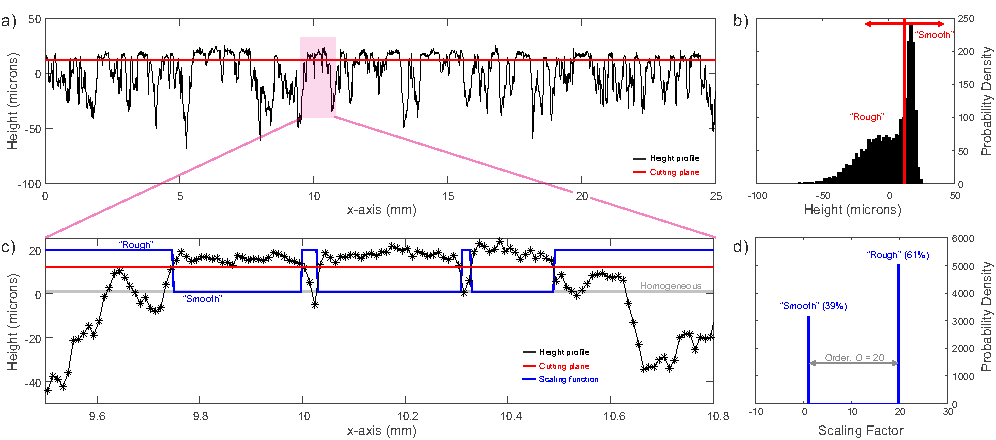
\includegraphics{FIG3.pdf} 
	\caption{ \textbf{(a)} 1-D roughness profile (black) taken from the transect at $y$ = 2 mm in Figure \ref{fig1}(f).  The cutting plane $h_{cut}$ = 5.8 $\mu$m is used to separate the bimodal distribution into smooth and rough surfaces. \textbf{(b)} PDF of the height profile in (a) with the cutting plane shown. \textbf{(c)} Small section of the height distribution showing the roughness profile (black line), the cutting plane (red line) and the scaling function (blue line). \textbf{(d)} PDF of the scaling function $\mathrm{SF}(x)$ with an order of heterogeneity $O$ = 20.}
	\label{fig3}
\end{figure}

A scaling function ($\mathrm{SF}$) is used to partition the smooth and rough sections of the fault. Figure \ref{fig3}(c) shows a detailed view of the roughness (black), the cutting plane (red) and the scaling function (blue). When the roughness was above the cutting plane we defined a scaling function ( $\mathrm{SF}$) to have value of unity. All heights below the cutting plane were prescribed as scaled value. This allowed us to control the magnitude of heterogeneity we call the `order'. For this example the order was $O$ = 20. The  $\mathrm{SF}$ produced heterogeneity in two manners: (\textit{i}) spatial variations were controlled by the location where the roughness profile crossed the cutting plane and ($ii$) the level (order) of heterogeneity -- the peak-to-peak range of SF -- was chosen by the modeler. The order of the $\mathrm{SF}(x)$ is clear seen in PDF in Figure \ref{fig3}(d).

We approach the model in a non-traditional manner and imposed heterogeneity primarily through the frictional critical slip-weakening variable $D_{c}(x)$. Spatial fluctuations in fault roughness -- smoother and more rough sections -- assumed properties based on arguments that follow past laboratory observations \citep{Marone1994}. Smooth sections are prescribed lower $(D_{c})_{low}$, and spatial fluctuations in critical slip distance was given the lower value multiplied by the scaling function $D_{c}(x) = (D_{c})_{low}\cdot$SF(x). The magnitude $D_{c}$ in the rough sections depended on the order $O$ of the scaling function. For example, for order $O$=20, the larger critical slip value was $(D_{c})_{high} = \textrm{max}[D_{c}(x)] =$ 25 nm$\cdot$ 20 = 500 nm = 0.5 $\mu$m. This assumption also follows micro-mechanical simulation governing friction on dry, gouge-free interfaces \citep{Yoshioka1996,Yoshioka1997}. 

\subsection{Frictional parameter space}
\label{ParameterSpace}
We choose parameters that are based on previous studies surrounding results from the experiment but we also incorporate assumptions from the literature. The goal of the models is to identify conditions that produce local seismicity -- a critical experimental observation made from the PZT sensors. In Figure \ref{fig4} we investigate how the critical nucleation length $L_{c}$ (equation \eqref{eq8}) varies with $D_{c}$ and the normal stress $\sigma$.  Based on experiments performed by \citet{Berthoude1999} for PMMA we set $a/b$ = 0.65 and $b$ = 0.0144. Curves representing constant critical nucleation length are shown in red for $L_{c}$ = 25 mm and 0.9 mm, for reference.   

\begin{figure}
	\centering
	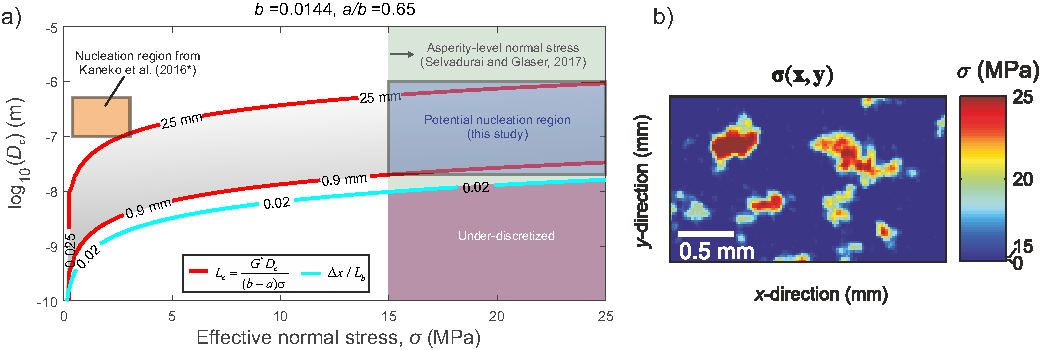
\includegraphics[scale = 0.95]{FIG4.pdf} 
	\caption{(a) Initial estimates of the nucleation parameter space ($L_{c}$) based on measurements of local normal stress \citep{Selvadurai2017}, minimum mesh discretization ($\Delta x /L_{b}$) and maximum critical nucleation size $L_{c} = 0.025$ m. The gray hatched region represents possible nucleation sizes for the mesoscopic length scale.  The hatched orange shows the ranges of $D_{c}$ and effective normal stress $\sigma$ that nucleated gross fault in \citet[][, *$a/b$ = 0.6944]{Kaneko2016}. (b) Example of asperity-level normal stress field measured using an experimental pressure sensitive film (adapted from \citet{Selvadurai2017}).}
	\label{fig4}
\end{figure}

To further constrain our models, we examined the experimentally measured asperity normal stress from the concerted study by \citet{Selvadurai2017}. Using the calibrated pressure film \citep{Selvadurai2015}, they found the asperities attained normal stresses ranging from $\sigma$ = 12 to 25 MPa. This range of normal stress is superimposed in Figure \ref{fig4}, which further bounds the potential nucleation conditions in our RSF model.

It was necessary to ensure that the fault was properly meshed to correctly capture the dynamic processes at the rupture tip during seismic events. Our calculations were based on the estimates of the cohesive (or breakdown) zone length scale $L_{b}$ in equation \eqref{eq8b}. To accurately capture local frictional breakdown it was necessary to apply a minimum grid size of $\Delta x/L_{b} <$ (1/50), which for $a/b$ = 0.65 was deemed acceptable.  In this model we choose to use 2$^{13}$ = 8192 grid points over the length $L$ = 25 mm of the mesoscopic domain, resulting in a resolution $\Delta x \sim$  3 $\mu$m. This is much different that the macroscopic parameter space estimated by \citet{Kaneko2016}, shown as orange hatched region, for the plastic-on-plastic sliding experiment performed by \citet{Latour2013}. Table \ref{table1} shows the baseline frictional, material and length scale parameters used in this study. More information on the convergence tests for the heterogeneous models is given in the Supplemental Information S1.

\begin{table}[ht]
	\centering
	\caption{General model parameters used in the 1-D RSF models.}
	\begin{tabular}{ m{5cm} m{2cm} m{4cm}} 
		\hline  
		\bf{Parameter} 			& \bf{Symbol} 		& \bf{Value}	\\
		Shear modulus  			& $G$  		 	& 2.39 GPa		\\
		Poisson ratio  			& $\nu$  	 	& 0.32 		\\
		Shear wave speed		& $V_{S}$      		& 1330 m s$^{-1}$	\\
		Reference friction coefficient	& $\mu$	        & 0.6	\\
		Reference slip rate  		& $V^{*}$     		&  0.1 $\mu$m s$^{-1}$\\
		Dynamic sliding threshold   	& $V_{dyn}$  		& 0.177 m s$^{-1}$ \\
		Loading plate velocity  	& $V_{LP}$     		&  0.1 $\mu$m s$^{-1}$\\
		Lower critical slip distance 	& $\left(D_{c}\right)_{low}$    &  25 nm\\
        Heterogeneous critical slip distance 	& $D_{c}(x)$    &  $\left(D_{c}\right)_{low} \cdot$ SF(x)\\
  		Normal stress 			& $\sigma$  		&  25 MPa \\
		Length of mesoscopic domain 	&   $L$  		& 25 mm\\
		Height of mesoscopic domain 	&   $H^{'}$  		& 2.5 mm\\
		Width of mesoscopic domain 	&   $W$   		& $\infty$\\
		Grid size 			& $\Delta x$ 		& 3 $\mu$m \\
		Grid points 			& $n$ 			& 2$^{13}$ \\
		RS parameter $b$ (VW)  		& $b$ 			& 0.0144  \\
		RS parameter $a$ (VW)  		& $a$ 			& 0.00936  \\
	    Simulation time 			& $t_{sim}$ 		& 600 s  \\
		\hline  	
	\end{tabular}
	\label{table1}
\end{table}

\section{Computational Results}

The general domain for the 1-D frictional model is shown in Figure \ref{fig5}(a). This represents the mesoscopic region of material under the eddy current target shown in Figure \ref{fig1}(c). The geometry of the domain is $L$ = 25 mm (corresponding to the extent of the roughness measurement in the direction of slip), $H^{'}$ = 2.5 mm (corresponding to the height of the material just below the eddy current target) and $W$ = $\infty$ (corresponding to plane strain conditions). The boundary element code QDYN assumes frictional properties ($a$, $b$ and $D_{c}$) and normal stress ($\sigma$) at each node on the interface. Figure \ref{fig5}(b) shows a schematic representation of the boundary value problem. A few representative nodes are shown as slider blocks. Communication between the frictional nodes is shown as spring elements. QDYN  solves the equation of motion given in \eqref{eq9}. Before moving to more complex, heterogeneous cases we examine the behavior of the homogeneous case to develop a baseline.    

\subsection{Homogeneous case}
From the mesoscopic geometry we build the 1-D homogeneous model, shown schematically in Figure \ref{fig5}(b). For the homogeneous case, each node has velocity-weakening (VW) conditions ($a-b$) = -0.005, $a/b$ = 0.65, normal stress $\sigma$ = 25 MPa and a critical slip-weakening distance $D_{c}$ = 25 nm. For the homogeneous case, the steady-state sliding velocity $V^{*}$ was assumed to be equal to the load point velocity $V_{LP}$. We were able to determine this experimentally from the near-fault slip velocity measurements made using the eddy current slip sensors shown in Figure \ref{fig1}(d) and  $V_{LP}$ = 0.1 $\mu$m/s  was used in this study.

\begin{figure}
	\centering
	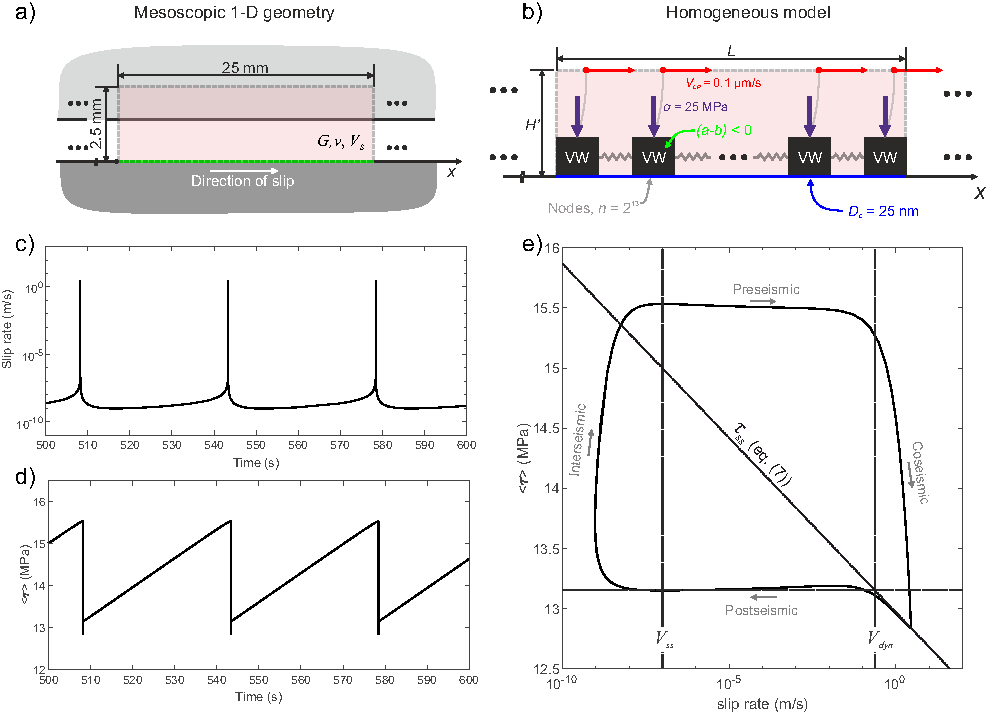
\includegraphics{FIG5_revised.pdf} 
	\caption{\textbf{(a)} General dimensions of the model domain described in Figure \ref{fig1}(c). \textbf{(b)} Description of the 1-D boundary value problem being solved by QDYN.  RS frictional behavior is described by equations \eqref{eq5} to \eqref{eq8}. \textbf{(c)} Average slip velocity and \textbf{(d)} average shear stress along the fault between $t_{sim}$ between 500 to 600s. We see that the fault underwent stick-slip behavior. \textbf{(e)} A diagram of the earthquake cycle for the VW fault that includes preseismic, coseismic, postseismic and interseismic phases.}
	\label{fig5}
\end{figure}

Each numerical simulation lasted for $t_{sim}$ = 600 s, which allowed for the fault to fully-develop a periodic stick-slip response \citep{Hillers2007}.  Figure \ref{fig5}(c) and (d) shows a small time window (500 to 600 s) of the slip velocity and shear stress, respectively, averaged over all nodes in the model.  We see that periodic ruptures are analogous to a `stick-slip' event. Over the full simulation, 18 stick-slip were recorded for the homogeneous case but only three are shown here.  Coseismic slip was defined when any node experienced a sliding velocity $V > V_{dyn}=$0.177 m/s as defined by equation \eqref{eq8c}. To further characterize the homogeneous case, Figure \ref{fig5}(e) shows the relationship between average slip velocity and shear stress which depicts the seismogenic evolution of the systems between different seismic regimes: interseismic, preseismic, coseismic and postseismic regime \citep{Ampuero2008}.

\subsection{Heterogeneous $D_{c}$-model}
We produce heterogeneity by varying the distribution of the critical slip weakening distance $D_{c}$ according to the scaling function ($\mathrm{SF}$) in Figure \ref{fig3}(c). The $D_{c}$-model shares some properties of the homogeneous case ($b$ = 0.0144, $a/b$ = 0.65, $\sigma$ = 25 MPa) and is depicted schematically in Figure \ref{fig6}(a). For the $D_{c}$-model we prescribe the lower value of critical slip weakening distance $(D_{c})_{low}$ = 25 nm. Using the scaling function from the cutting plane method, we can capture the spatial variation in critical slip weakening distance given as $D_{c}(x) = (D_{c})_{low} \cdot \mathrm{SF}(x)$. Figure \ref{fig6}(b) shows the spatial fluctuations in $D_{c}(x)$ for heterogeneity on the order of O20. Spatial distribution of the homogeneous properties is shown in Figure \ref{fig6}(c) for reference.
 
The average slip rate and shear stress for this $D_{c}$-model (O20, blue) is shown in blue in Figures \ref{fig6}(d) and (e), respectively. For reference, we also show the results from the homogeneous model O1 (black). We see that the fault does experience some stick-slip behavior -- the small spikes in slip velocity -- but it does not experience full ruptures with large levels of shear stress drop that occurred in the homogeneous case. 

 \begin{figure}
	\centering
	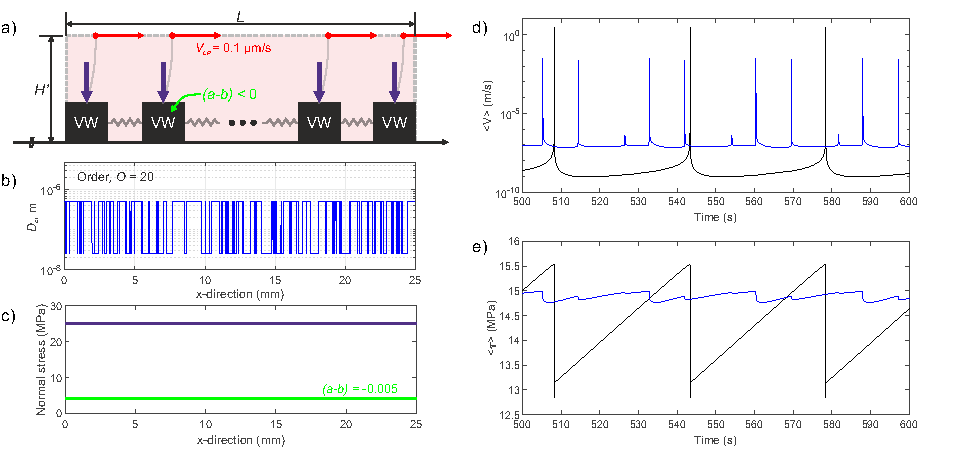
\includegraphics{FIG6_revised.pdf} 
	\caption{\textbf{(a)} General schematic showing the heterogeneous model. \textbf{(b)} Heterogeneous distribution of $D_{c}$, with O20. \textbf{(c)} Constant normal stress and VW rheology ($a-b <$ 0) is shown along the $x$-axis.  \textbf{(d)} Average slip velocity is shown along the fault for the heterogeneous model (blue line), which is compared to homogeneous model (black line). \textbf{(e)} Phase diagram between shear stress and slip velocity for heterogeneous and homogeneous models.}
	\label{fig6}
\end{figure}
 
We investigated the effect of different levels of heterogeneity. In Figure \ref{fig7} the average fault behavior is shown for three levels O10 (red), O15 (green) and O20 (blue), which all use the same scaling function $\mathrm{SF}(x)$.  This is again compared to the average behavior of the homogeneous fault O1 (black).  The average slip, slip rate and shear stress is given in Figures \ref{fig7}(a), (b) and (c), respectively.  We observed an increase in complexity from homogeneity with these models. The first major note is that both O10 (red) and O15 (green) still experienced full system wide rupture (large events that propagated the full extent of the modelled fault).  Full rupture would nucleate from a smooth section of the fault and would not always arrest when compared to more localized ruptures that occurred in the O20, which had stronger barriers. 

We see that along with system-wide events, O10 (red) and O15 (green) also experienced small localized events that were arrested by the neighbouring barriers. These were denoted as ``foreshock sequences'' leading up to the mesoscopic main rupture (larger stress drop on system-wide events), which highlighted in Figure \ref{fig7}(c). We clearly see that as the order O is increased, the fault exhibits transition from well-behaved fault (homogeneous, O1) to relatively chaotic mixture of system wide events with small localised ruptures (O10 and O15), then returning to well-behaved creep-dominated fault with small localized events on a preferential patch (O20).

\begin{figure}
	\centering
	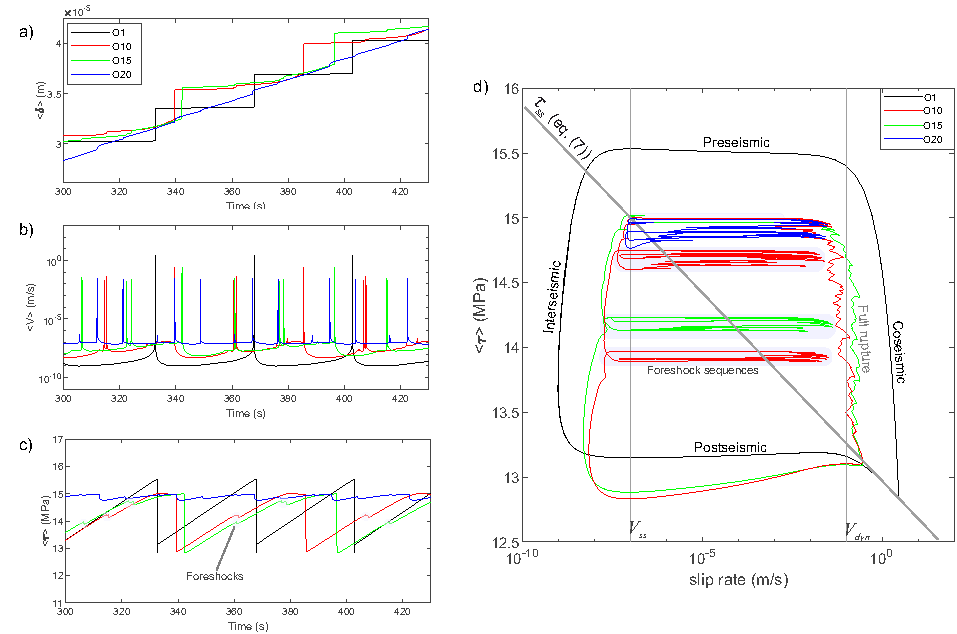
\includegraphics{FIG7.pdf} 
	\caption{Three heterogeneous models $O$ =  10 (red), 15 (green) and 20 (blue) are compared to the homogeneous model (black) for a short time window between 300 and 430 s. We show the \textbf{(a)} average slip, \textbf{(b)} average slip velocity and \textbf{(c)} average shear stress.  We highlight where small drops in shear stress were seen and relate them small localized events (foreshocks). \textbf{(d)} We examine the phase diagram between shear stress and slip velocity for each heterogeneous model in comparison to the homogeneous model.}
	\label{fig7}
\end{figure} 

To better visualize the systems behavior, we plot all models on phase-diagrams described in Figure \ref{fig5}(e) for the homogeneous case. The average fault behavior cycles from co- to post- to inter- to pre-seismic, moving around $\tau_{ss}$ given in equation \eqref{eq7}. The O10 (red) and O15 (green) models appear to observe, in general, lower total stress drop during the full rupture events when compared to the homogeneous case.  We also see that during a full rupture, the average slip rate on these faults is in general lower than the homogeneous case.  For the most heterogeneous fault with order O20, we see that full rupture events did not occur but there was some deviation from steady state caused by small foreshock sequences that deterred the fault from simply `creeping' along at the steady state shear stress. 

We see these foreshock sequences highlighted in the phase diagram (gray regions). Two major sequences were observed for the O10 and O15 models. Timing of these foreshock sequences, relative to the full fault cycle, are shown for O10(red) and occurred in the interseismic stages of the main rupture cycle. For O15(green), one foreshock sequence occurred in the interseismic portion and one closely after the fault entered the nucleation phase of the larger rupture cycle. As for O20 (blue), this smooth section of the fault prone to localized rupture behaved in a relative synchronous manner. More details to the spatio-temporal complexity of these ruptures are given in the next section. 

\subsubsection{Spatio-temporal behavior or precursory seismicity }
\label{spatialmodel}

In Figure \ref{fig8} we examine the spatio-temporal evolution of the $D_{c}$-model with O17.5. We note that this model was not presented in the previous section. The purpose of the previous section was to highlight changes in the general fault behavior at three levels of heterogeneity  with distinctly different behavior. All spatio-temporal distributions of slip are shown in a similar manner in Supplemental Sections S3 for all models in this study.

Figure \ref{fig8}(a) shows the spatio-temporal evolution of slip along the fault from time $t$ = 300 s to 600 s. The time step between each isochron was uniform, taken every 30 intervals of adaptive time steps.  We note that if any point on the fault slipped rapidly, the adaptive time step would decrease to accurately solve the boundary value problem. Seismicity (red slip isochrones) was defined as any node in the model experiencing slip velocities $V > V_{dyn}=$0.177 m/s. Below this threshold the fault was assumed to be sliding aseismically (blue slip isochrones). Using this description we were able to clearly identify certain `seismic patches'.

One patch is highlighted in Figure \ref{fig8}(a) and enhanced in (c) where we examine slip on the transect $x$ = 5 to 8 mm from $t$ = 300 s to 305 s.  This asperity section of the fault was prone to seismicity in all models, even the O20 that showed limited localized seismicity and is referred to a the \textit{dominant asperity}. Figure \ref{fig8}(b) shows the spatial variability in heterogeneity in $D_{c}$ along that section (for this case with O17.5). In Figure \ref{fig8}(c), we see that the fault slips aseismically between ruptures which delineates the seismicity over these five seconds. Four individual ruptures are shown and these events exhibit crack-like behavior but remain complex throughout the extend of the simulation due to the spatial variability in $D_{c}$, the level of heterogeneity (O17.5) and the continuously evolving shear stress on the fault.

In Figures \ref{fig8}(d) and (e) we investigate the space-time plot of slip velocity and shear stress, respectively, for Event 4 in the asperity failure sequence. The portion of the fault is shown ($x$ = 5 to 8 mm) and we have superimposed the heterogeneity from Figure \ref{fig8}(b) for clarity. We see that Event 4 nucleates at the edge of a `smooth-rough' boundary ($x \sim$ 7.25 mm) depicted as the purple star. As the rupture expands, it propagates bi-laterally at different rates. We have superimposed three lines of constant velocity 0.5$\cdot V_{S}$ (green), $V_{S}$ (red) and $V_{P}$ (blue).  Upon nucleation, the rupture expands outward in a subsonic manner, moving faster ($\sim 0.75 \cdot V_{S}$) ``up-strike'' into the smoother, less resistive section than into the ``down-strike'', rougher and more restive section ($\sim 0.45\cdot V_{S}$). This behavior represented typical rupture behavior for localized events on the dominant asperity.

\begin{figure}
	\centering
	\includegraphics[scale = 0.95]{FIG8_revised.pdf} 
	\caption{\textbf{(a)} Complex rupture for a fault with heterogeneity order $O$ = 17.5. Slip along the fault is shown for isochrones when the fault was sliding seismically (red, $V_{dyn}>$ 0.177 m/s) or aseismically (blue, $V <$ 0.1m/s).  Results are only shown for simulations times between $t$ = 300 s and 600 s. We use these results to calculate the properties of the localized ruptures that showed local nucleation, dynamic rupture and arrest behavior due to heterogeneity in $D_{c}$. \textbf{(b)} We show spatial heterogeneity for a dominant asperity of the fault from $x$ = 5 to 8 mm. \textbf{(c)} We look at a small sequence composed of four individual ruptures between time $t$ = 300 s to 305 s on the dominant asperity.  We see that the rupture has complex distributions of slip and spatio-temporal distributions. To better understand the temporal changes of the rupture we show the spatio-temporal evolution of Event 4 in terms of its \textbf{(d)} slip velocity and \textbf{(e)} shear stress.}
	\label{fig8}
\end{figure}

Spatio-temporal rupture evolution for Event 4 is enlarged in Figure \ref{fig9}(d).  We see more clearly the subsonic rupture propagation that grows bi-laterally at different rates until arriving at separate barriers. Once the up-strike crack-tip (i.e. that moving on the smooth fault) reached an up-strike barrier, it was abruptly arrested (shown as the red star).  As this rupture is arrested a back propagating front is emitted moving closer to the P wave velocity.  This front is known as the P stopping phase.  This stopping phase was observed by \citet{Madariaga1976} during numerical simulations studying the kinematic behavior of a circular asperity.  In that problem, the $P$ stopping phase is the wave radiated when the rupture front suddenly stops (red stars), for example when encounters a strong enough barrier.  Both the up- and down-strike rupture encountered barriers and produced separate $P$ stopping phases.  For the down-strike propagating crack-tip, this $P$ stopping phase actually caused the overall dimension of the to grow larger, finally stopping at the green star. 

To estimate properties of each rupture we used an image detection algorithm (regionprops \citep{Matlab}) and examined the 2-D distance-time space. Using the slip velocity threshold of $V_{dyn}>$ 0.177 m/s, the ruptures were easily separated and properties such as the half-length $L_{r}$ is shown in Figures \ref{fig9}(d).

A purpose of this study is to characterize and compare source properties to those reported kinematically by \citet{Selvadurai2019}. We developed tools to quantify the cumulative slip ($\delta$), RSF stress drop ($\Delta \tau$) and effective fracture energy ($G^{'}$) and rupture half-length ($L_{r}$) for each rupture as to account for their individual complex behavior.

\subsubsection{Constitutive behavior of individual ruptures }
\label{Constitutive}
In Figure \ref{fig9} we look at the complex behavior of Event 4 from the previous section.  In Figure \ref{fig9}(d) we show an enlarged view of Event 4 that ruptured a section with linear rupture dimension $2L_{r}$.  To better understand the complex behavior of all seismic rupture moving forward, we divide the full length of the rupture into 25 equally spaced points along the $x$-axis. The number of transects used was sufficient to sample ruptures and a sensitivity study investigated the number of required sampling transects is discussed in Supplementary Section S2.   

\begin{figure}
	\centering
	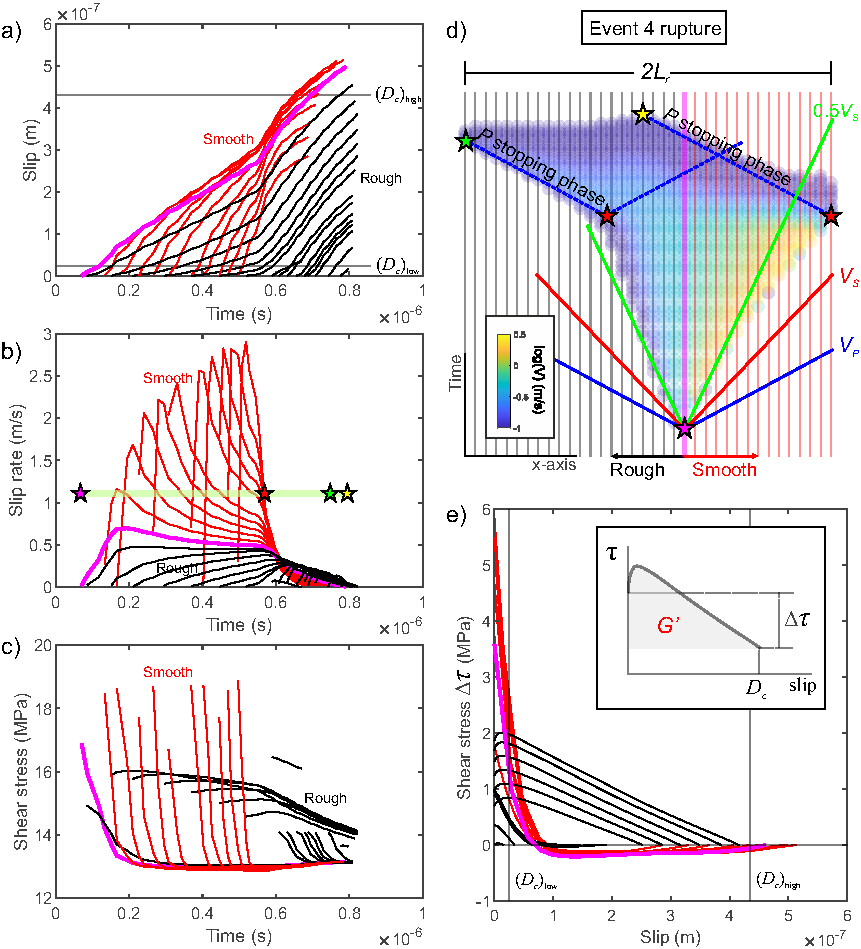
\includegraphics{FIG9.pdf} 
	\caption{Rupture complexity of Event 4 in Figure \ref{fig8}(d) and (e) in space-time plots.  \textbf{(a)} Temporal evolution of slip along 25 different transects of the rupture spaced evenly on the fault. \textbf{(b)} Temporal evolution of slip rate along the same transects as in (a). Key moments of the rupture are given by the colored stars. \textbf{(c)} Temporal evolution of shear stress for the same positions as in (a). \textbf{(d)} Space-time plot of the rupture with the transects depicted graphically. \textbf{(e)} We investigate the traction-slip from each transect. The inset image shows how we measure (static) stress drop ($\Delta \sigma$) and effective fracture energy ($G^{'}$) for each position on the fault.}
	\label{fig9}
	
\end{figure}
In Figure \ref{fig9} we provide concise temporal understanding showing the diversity in the temporal evolution of: (a) slip, (b) slip-rate and (c) shear stress along the spatial transects of Event 4. In Figure \ref{fig9}(a) we observe that the rupture has a non-uniform distribution of accumulated slip. The average slip along the 25 estimates was $\delta$ = 0.37 $\mu$m.  We use this to estimate the scalar seismic moment $M_{0}$ given by \citet{Aki1966}: 
\begin{equation}
M_{0} = G A \delta, 
\label{eq9}
\end{equation}
\noindent where $A$ is the fault area and $\delta$ is slip. For a penny-shaped fault $A$ = $\pi r^{2}$ and for a square fault $A$ =$(2L_{r})^{2}$. Using this estimate the scalar seismic moment $M_{0}$ = 0.0014 N$\cdot$m. This is equivalent to a moment magnitude $M_{w} = (2/3)\cdot(log_{10}(M_{0})-9.05) = -7.94$ \citep{Kanamori1975}.  Transects were color coded for the smooth (red) and rough (black) sections of the fault to highlight the differences in their dynamic response. As expected the rougher sections showed higher variability in cumulative slip along each transect since they were responsible for arresting the rupture.    

Slip rate along each transect is shown in Figure \ref{fig9}(b). For further clarity, important times of the rupture are shown as colored stars and are superimposed. We can see that the rupture has higher slip rates along the smoother section of the fault, whereas the rough section offers more resistance and slip rates are lower. Shear stress along each transect is shown in Figure \ref{fig9}(c). Smooth portions of the fault (red lines) achieve higher peak stress and exhibit higher weakening rates than the rough sections (black lines), which offer higher resistance to rupture.

Figure \ref{fig9}(e) shows the slip-traction relationship for each transect. Values are normalized is with regards to the final stress and using the inset image we can calculate stress drop ($\Delta\tau$) and effective fracture energy ($G^{'}$).  The latter is also known as breakdown work in the literature \citep[e.g.,][]{Tinti2005, Cocco2016}. We see that there are clear differences in the participation of each surface (rough and smooth) in the metrics that have be extracted. 

For clarity we have highlighted the critical slip weakening distance for both the smooth $(D_{c})_{low}$ and rough section of the fault $(D_{c})_{high}$. We see that in some cases slip was greater than $(D_{c})_{high}$ which can be explained as dynamic overshoot \citep{Madariaga1976}. Calculating $\Delta \tau$ is relatively straight forward, but to determine the effective fracture energy $G^{'}$, we numerically integrated the area under this curve. For Event 4, the average stress drop was $\Delta\tau$ = 3.25 MPa and average effective fracture energy $G^{'}$ = 0.13 J/m$^{2}$.  

\subsection{Summary of precursory source properties}
\subsubsection{Seismic moment versus source size}
In Figure \ref{fig10}(a) we examine the relationship between source area $A_{r} = (2\cdot L_{r})^{2}$ and seismic moment $M_{0}$ for the different RSF models. Source properties determined in the previous section are compared to those inferred from seismic waves from a concerted study by \citet{Selvadurai2019}. We show the results five $D_{c}$-models (circles) against the kinematic estimates detailed by \citet{Selvadurai2019} from the P and S waves.  Full ruptures referred to events that ruptured the entire fault surface. RSF ruptures followed the routinely observed empirical scaling relationship between seismic moment and source geometry ($M_{0} \propto L_{r}^{3}$). Figure \ref{fig10}(c) shows the relationship between stress drop and seismic moment, which was relatively constant $\sim$ 1.86 MPa where smaller rupture had slightly lower values of stress drop.

\begin{figure}
	\centering
	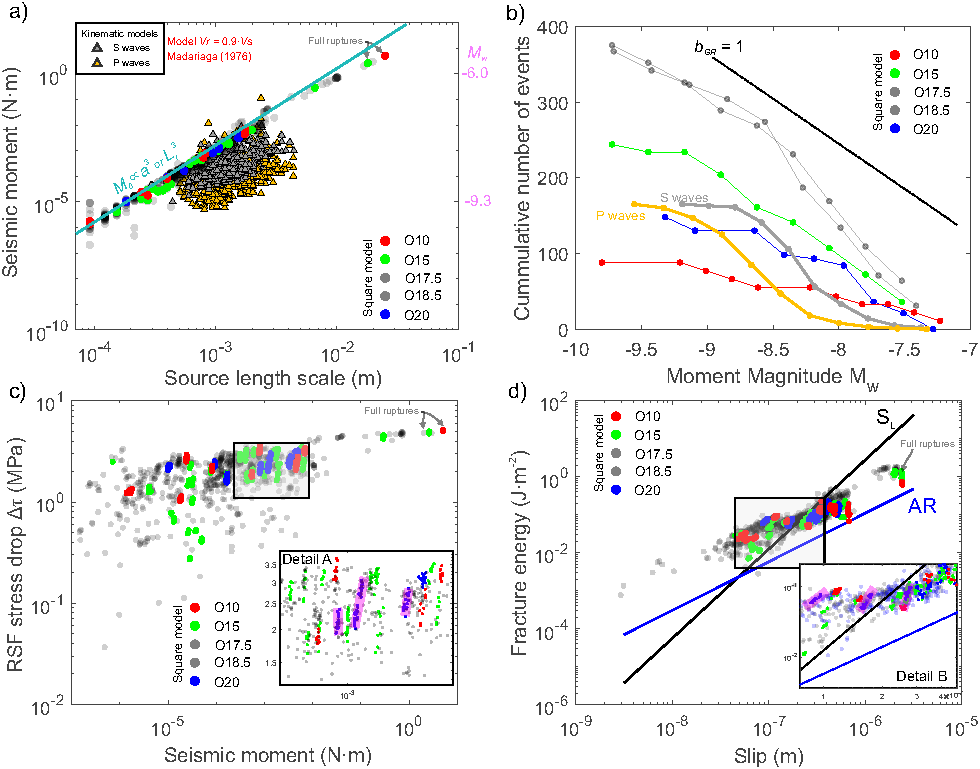
\includegraphics[scale = 0.95]{FIG10_revised.pdf} 
	\caption{\textbf{(a)} Source length scale is calculated from the numerical models with various levels of heterogeneity (colored circles) and compared to their respective scalar seismic moment $M_{0}$. These are compared to the kinematic estimate of source properties determined using shear crack models described in \citet{Selvadurai2019} for both P and S waves (triangles). \textbf{(b)} Frequency-magnitude distributions (FMDs) are given for each catalog shown in (a). A reference value of  $b_{GR}$ = 1 is shown for reference. \textbf{(c)} Relationship between stress drop ($\Delta\tau$) and ruptured area $M_{0}$. \textbf{(d)} Effective fracture energy ($G^{'}$) versus slip is shown. We compare the models to empirical scaling estimates from laboratory seismicity \citep[black line,][]{Selvadurai2019} and field estimates \citep[blue line][]{Abercrombie2005}, in which the latter has been extrapolated.}
	\label{fig10}
\end{figure}

\subsubsection{Frequency-magnitude distribution}
Estimates of the frequency-magnitude distributions (FMDs) from the kinematic estimates and the RSF model are shown in Figure \ref{fig10}(b). The colors are the same as legends in Figure \ref{fig10}(a).  The Gutenberg-Richter \citep{Gutenberg1944} law is the most commonly observed empirical relationship in seismology.  It states that large earthquakes occur less frequently than small earthquakes following the standard relationship $log_{10}(N)= a_{GR} - b_{GR}M_{w}$, where $N$ is the number of events equal or above magnitude $M_{w}$ and $a_{GR}$ and $b_{GR}$ are constants describing the productivity and\textbf{ sizes of }earthquakes, respectively\cite[e.g.][]{Wiemer2002}.  

Figure \ref{fig10}(b) shows FMDs and $b_{GR}$ = 1 is shown for reference. We see that the model produced definite changes in the slope of the distribution.  The productivity $a_{GR}$  is relatively low for O10 (red), O15 (green) and O20 (blue) models and O17.5 and O18.5 (gray) show the highest level of productivity. On simulation with lower relative heterogeneity, i.e. the ``smoother models'' (O10 and O15), the b-value $b_{GR} < 1$ suggesting there are similar amounts of small to large earthquakes.  $b_{GR} \sim 1$ on faults where the relative heterogeneity was increased O17.5 and O18.5 but then dropped again for O20. We note $b_{GR}$ = 1 as shown only as reference since FMD are likely be distorted by scale-variant behavior imposed by a length scale-dependent physical processes that will be discussed in later.

\subsubsection{Fracture energy scaling}
\label{FracEnergy}
Scaling behavior between effective fracture energy $G^{'}$ and slip $\delta$  is compared to the  empirical relationship $G^{'} \propto \delta^{\gamma}$. In Figure \ref{fig10}(d) estimates of $G^{'}$ for the different models are shown. These are compared to the previously discussed empirical relationship for shear crack source models from laboratory ($S_{L}$, $\gamma = $2.35) \citep{Selvadurai2019}  and estimates made at regional scales from natural earthquakes (AR, $\gamma = $1.28) following the observations by \citet{Abercrombie2005}.  We see that the results from the model tend to follow the same slope as AR but if we look more closely, at Detail B, we see that some of the repeating patches show steeper trends in scaling. This can be explained by the fact that the preferential worn patches would remain relatively constant in size but the stress drop varied as is shown in Detail A in Figure \ref{fig10}(b).

\subsubsection{Recurrence rates}
\label{Recurrence times}
In Figure \ref{fig11}(a) we show the average slip (black) and average shear stress (red) for a 100 s of the simulations for strong barriers O20 (left-hand side, LHS) to weaker barriers O10 (right-hand side, RHS) and the transitional case O17.5 (middle panel).  We see the general behavior of the fault transitioned from one that is creep-dominated (O20) to one that stick-slip dominated (O10). Creep-dominated and stick-slip dominated is defined by how much the average slip deviates from the creeping rate ($V_{creep} = t\cdot V_{LP}$). 

We look recurrence rate $T_{r}$ for the localized events in each model which is considered to be the time between any two events at any location on the fault. To disseminate triggered  seismicity (e.g. aftershock) versus isolated events, we adopt the methodology described in \citet{Lengline2009}. They looked at the probability distribution function (PDF) of the recurrence times and normalized by the average recurrence time $T^{*}_{r}$.  They found that events below $T_{r}/T^{*}_{r} <$ 0.1 follow a power-law distribution consistent with Omori's law that described aftershocks in nature \citep[e.g.,][]{Lengline2009}. 

In Figure \ref{fig11}(b) we show the probability distribution of $T_{r}/T^{*}_{r}$ for the five $D_{c}$-models. The purple region highlights portions of the distribution that are not triggered events according to \citet{Lengline2009}. We see that for the creep-dominated O20 model there is relatively equal probability in recurrence time but a slight increase in  $T_{r}/T^{*}_{r} >$ 0.1 promoting the idea these events are not triggered and are the results of the overall loading of the fault. In the transitional models (O18.5, O17.5 and O15) we fit a power law distribution (gray lines) between 1e-5 $< T_{r}/T^{*}_{r} <$ 0.1 and found its slope to decrease as the heterogeneity was decreased. We note a small `bump' in probability above $T_{r}/T^{*}_{r} >$ 0.1, denoted with the small arrow in O15. This appears to have been amplified in O10, or the stick-slip dominated model, and this is discussed later in conjunction with the results surrounding the FMDs.  This may be related to cascade-up foreshock behavior (see Discussion Section \ref{Cascade_UP}) but this will likely require more rigorous investigation.

\begin{figure}
    	\centering
	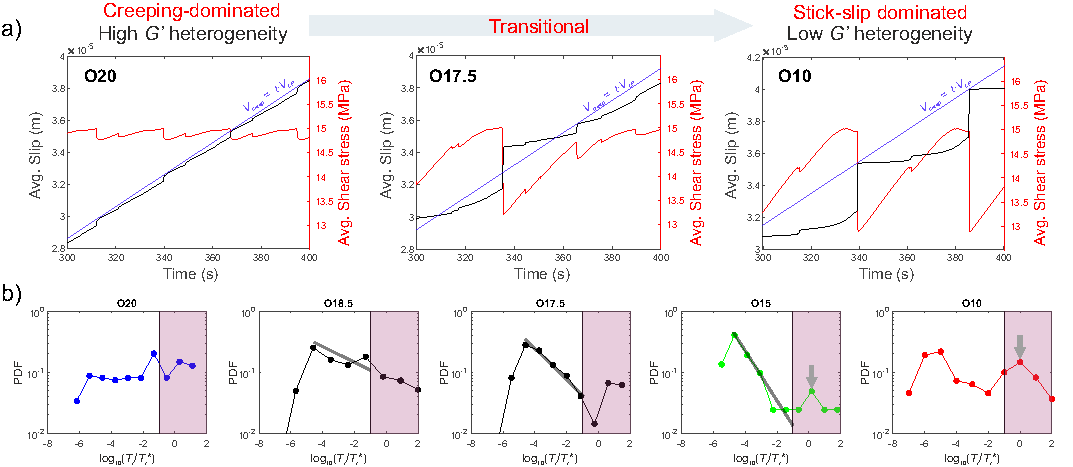
\includegraphics[scale = 0.9]{FIG11_revised.pdf} 
	\caption{Earthquake recurrence rate for each $D_{c}$-model from higher O20 to lower O10 levels of strength heterogeneity. (\textbf{a}) We show the average behavior of the entire fault for small portion of time $t$ =300 to 400 s for the O20 (creeping-dominated), O17.5 (transitional) and O10 (stick-slip dominated) models. (\textbf{b}) Probability distribution functions of the lognormal distribution of normalized recurrence rates $T_{r}/T^{*}_{r}$ for all models. The probabilities above $T_{r}/T^{*}_{r} >$ 0.1 in purple are highlighted.}
	\label{fig11}
\end{figure}
\subsection{Heterogeneous \textit{Composite}-model}
The primary goal of this study is providing an understanding of what types of RSF heterogeneity could help explain a suit of experimental observations. The prior models have employed heterogeneity with a minimal level of unknown variables. We increase the complexity of the model using a \ital{Composite}-model.  This version of our model aims at illuminating an additional complexity that may exist spatial distribution in normal stress. This model is presented in the aim of expanding the possible boundary conditions that can feasibly explain concomitant slow and fast slip on a frictional interface. 

While this needs more investigation, this is version of our model is motivated by the experimental observations with made with the pressure sensitive model (Figure \ref{fig4}(b)) that normal stress heterogeneity also exist \citep{Selvadurai2017}. To model such conditions, we again use the scaling function. However, now on smooth sections (low $D_{c}$) we prescribe constant normal stress $\sigma_{high}$ = 25 MPa.  In rough sections, we apply a constant low normal stress level, which was set to the lower measurable limit of the pressure sensitive film $\sigma_{low}$ = 12 MPa \citep{Selvadurai2015a}. 

Figure \ref{fig12}(a) shows a section of the spatial heterogeneity on the dominant asperity in normal stress $\sigma$ (red) and critical slip weakening distance $D_{c}$ (blue).  The scaling function was chosen to be O20, which was a model that had a relatively well-behaved response from before.  We use the same methods to calculate source properties and examine similar relationships for this composite-model (O20C).

\begin{figure}
	\centering
	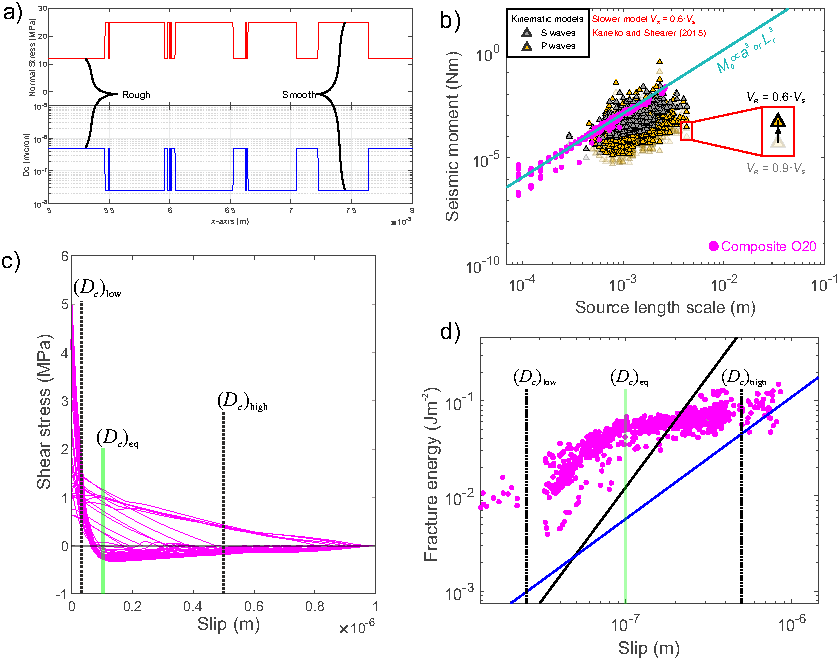
\includegraphics{FIG12_revised.pdf} 
	\caption{Results from the \textit{Composite}-model. \textbf{(a)} A small section of the 1D fault form $x$ = 5 to 8 mm showing the spatial variation in both $D_{c}$ and $\sigma$. \textbf{(b)} The scaling relationship between $A_{r}$ and $M_{0}$ (gray circles) is compared to the corrected kinematic estimates of source properties from \citet{Selvadurai2019} (triangles).   \textbf{(c)} Constitutive behavior for a large event in the \textit{Composite}-model. \textbf{(d)} Relationship between effective fracture energy $G'$ and slip $\delta$. Empirical relationship between black and blue lines is similar to the one shown Figure \ref{fig10}(d).}
	\label{fig12}
\end{figure}

Figure \ref{fig12}(b) shows the relationship between $M_{0}$ and $A_{r}$. We find that it produces similar estimates to the kinematic shear crack model shown in Figure \ref{fig10}(a). However, here we have made an additional improvement assumptions in the shear crack model regarding the rupture speed.  We now apply a correction factor to account for slower ruptures in the kinematic models for example $V_{r} = 0.6\cdot V_{S}$.  This analysis was performed by \citet{Kaneko2015} for a range of rupture scenarios: circular or elliptical and symmetric or asymmetric.  They found that decreasing the rupture speed can produce deviations of up to 2.5 times more stress drop depending on the model and the wave phase (P or S).  Average RSF estimates of rupture velocities were much lower 0.6$\cdot V_{S}$.  From table 1. in \citet{Kaneko2015}, we updated the estimates form \citet{Selvadurai2019}, which minimized the difference between the kinematic (triangles) and RSF (circles) estimates of source properties.  The correction factor used to scale the original kinematic estimates were taken from asymmetric circular asperity model for a rupture velocity $0.6\cdot V_{S}$ that led to an increase in seismic moment of 2.63 and 2.74 from P and S waves estimates, respectively.  Asymmetry in the rupture propagation was inferred from Figure \ref{fig9}(d).

Figure \ref{fig12}(c) shows the constitutive shear stress versus slip behaviour for a large random asperity. For reference, we mark the levels of $(D_{c})_{low}$, $(D_{c})_{eq}$ and $(D_{c})_{high}$.  The term $(D_{c})_{eq}$, or equivalent critical slip weakening distance, appears to be a representative critical slip weakening distance that always lies between the two $D_{c}$ limits but will likely vary on each rupture and is a function of the ratio of high to low resistance of the interface participating in rupture. Looking at the relationship between $G^{'}$ and slip. We see that the relationship appears to have a ``kink''.  This kink is observed about slip level of  $(D_{c})_{eq}$. 

\section{Discussion}
We have summarized findings from a well-documented laboratory experiment \citep{Selvadurai2015, Selvadurai2017, Selvadurai2019} that displayed complex nucleation behavior: preparatory slow preslip accompanied with intermittent localized seismicity from the same sections of the frictional interface (see Figure \ref{fig1}). A RSF model was developed to examine the complex frictional behavior using the rate- and state-dependent constitutive framework. The model accounted for wear that was observed from \textit{a posteriori} measurements of roughness on the slider block surface that was well characterized in terms of a bimodal Gaussian distribution of surface roughness (Figure \ref{fig2}(a)) -- an observation that has been well-documented in the field of tribology. Attributes of our worn interface show a distinct polished surface embedded in a rougher surface, a feature that may be similar to the polished fault mirrors (FMs) observed on natural outcrops (see Figures \ref{fig2}(e) and (f)).

A cutting plane method (Figure \ref{fig3}) was used to mathematically quantify the spatial variation between the smooth and rough sections. Two sets of RSF properties were chosen based on the fact that smooth surfaces have lower critical slip weakening distance $D_{c}$ than rougher sections and the level of heterogeneity was investigated. The models showed complex behaviour (Figure \ref{fig7}) that differed from the homogeneous case (Figure \ref{fig5}) that could explain the experimental observation of concomitant slow slip and the localized seismicity.  We developed algorithms to isolate ruptures (Figures \ref{fig8} and \ref{fig9}).  These allowed us to estimate a range of source properties, such as scalar seismic moment ($M_{0}$), rupture length scale ($L_{r}$), seismic slip ($\delta$), stress drop ($\Delta\tau$), fracture energy ($G'$), frequency-magnitude distributions (FMD) and recurrence rates ($T_{r}$) of five different $D_{c}$-models and a composite-model (Figures \ref{fig10}, \ref{fig11} and \ref{fig12}). These calculations were compared to independently estimated seismological source properties made from interpreting the seismic waves \citep{Selvadurai2019}

\subsection{`Cascade-up' nucleation behavior}
\label{Cascade_UP}
Our model exhibits a wide range of behavior ranging from relatively simple to chaotic (see Figure \ref{fig7}). In Figure \ref{fig5} we see that the homogeneous rupture is well-behaved, exhibiting regular stick-slip events at constant recurrence time.  In the model, we assume periodic boundary conditions. This implies that if a rupture is not arrested in the mesoscopic region and reaches boundary it would theoretically continue to rupture the macroscopic region -- cascading-up and creating a system wide event that was observed experimentally shown in Figure \ref{fig1}(b). 

We referred to these as full-ruptures and these are linked to cascade-up nucleation processes. This assumption is plausible when looking at the hypocenter of the full-fault rupture (i.e. system-wide stick-slip event) measured experimentally in \citet{Selvadurai2015}. It was consistently located in the region near the roughness measurement \citep[magenta star in fig. 7 and 8 in ][]{Selvadurai2015}. In Figure \ref{fig11} the two types of end-member behaviors are shown: 'creep dominated' and 'stick-slip dominated'. Stick-slip dominated behavior is described as supporting localized foreshocks but also small events would cascade-up and triggered full ruptures. Creep dominated would observe localized events but they never developed large stress drop full ruptures. The $D_{c}$-models O10 and O15 exhibited both foreshock sequences that were followed by cascade-up into full ruptures (Figure \ref{fig5}), whereas O20 and showed constrained ruptures that did not cascade-up. 

Heterogeneity between the O10 and O20 models is defined by variations in the weakening rate on each each region due to the constant level of normal stress along the fault, which, by definition, leads to spatial variations in fracture energy as defined in Section \ref{FracEnergy}. Our models suggests that relatively lower levels of heterogeneity in the fracture energy between the rough and polished sections create the stick-slip dominant behavior (foreshocks that can potentially cascade-up) and, once the heterogeneity is relatively large enough, a creep-dominant behavior is observed. Hierarchical heterogeneity in fracture energy has been proposed by others \citep{Ide2005, Aochi2014, Aochi2017} and will be discussed later.

While we cannot confirm an exact wear mechanism that would increase the level heterogeneity between smooth and rough sections with increased slip, a hypothesis is that certain sections of the fault are more prone to flattening (ironing) and others will develop particles of gouge. Flattening, or ‘ironing’, of asperities due to adhesive wear has recently been investigated using a material independent framework \citet{Aghababaei2016}. Physics-based numerical simulations found a critical length scale describing the deformation mechanisms of interacting asperities. At length scales below a critical value, asperities flatten inelastically and this was dependent on the size of the asperity junction, the work of adhesion of the bulk material, and the maximum elastic strain energy that can be stored at a contact. At length scales above this critical value, gouge-like material will form which has been found to also increase the critical slip-weakening distance in laboratory studies \citep{Marone1998}.   

\subsection{Dominant asperity}
All models appeared to hinge about the behavior of the heterogeneity highlighted on the section of the fault from $x$ = 5 mm to 8 mm shown in Figure \ref{fig8}(b) and (c). In all models, this section produced localized events. With lower levels of heterogeneity (O10 and O15) this produced both foreshocks and events that cascaded-up, rupturing the whole fault. In Supplemental Sections S3, we show spatio-temporal evolution of slip of O10 and O15 full-ruptures which breakdown in a similar manner -- nucleating each time from the from the dominant asperity.

This type of behavior may explain the observations in the Naka-Oki region in eastern Japan \citep{Okuda2018} and the Tohoku–Hokkaido subduction zone, Japan \citep{Ide2019}. These observations show that earthquakes shared almost identical growth patterns for repeating earthquakes of various sizes. If this observation follows our model, a explanation is that the repeater asperities that routinely produce  $M_{w} \sim$ 2  could have lower values of fracture energy (or $D_{c}$) that sometimes cascades-up to  $M_{w} \sim$ 4.8 \citep{Okuda2018a}.  They hypothesize that a hierachical structure exists as depicted in fig. 5 of \citet{Okuda2018}, which might be due to heterogeneity in the fracture energy \citep{Ide2005, Aochi2014, Aochi2017}. Our model agrees with this and heterogeneity is provided in the form of polished fault mirrors. 

Using a penny-shaped \citet{Eshelby1957} stress drop model $\Delta\sigma$, we can estimate the source radius as $a_{r} = \sqrt[3]{(7/16)(M_{0}/\Delta\sigma)}$, for an $M_{w}$ = 2. If we assume stress drops between $\Delta \sigma  = $ 1 MPa and 10 MPa, we find that the source radius to vary between $a_{r}$ = 36.5 m to 78.5 m.  While these seems to be very large, there have been cases of such large exposures of FMs on the active normal faults in central Greece \citep{Jackson1999}. These sizes of these FMs could explain the smaller $M_{w}$ = 2 repeater events in the Naka-Oki region of Japan.  

Another feature regarding the dominant asperity surrounded its unlocking sequence as shown in Figure \ref{fig8}(c). For clarity, the temporal unlocking sequence for the O17.5 model were enumerated in ascending order from 1 to 4.  Below the spatio-temporal slip evolution (red and blue isochrons), we show the spatial length of each rupture for clarity. We see each rupture overlaps the previous rupture. This phenomena was also observed by \citet{Okuda2018a} and was referred to as 'streaking', which is explained by patches of differing sizes possessing some hierarchical distribution. This also might be similar to the dynamic precursor detachment fronts observed experimentally on fault analogs \citep{Rubinstein2004,Rubinstein2006}. \citet{Okuda2018a} attribute the differences in small and between these small and large earthquake to subtle differences in physical conditions -- for our model this was due the presence of the fault mirrors which is linked to seismicity in our model.

\subsection{Repeating-like behavior}
In contrast the cascade-up behavior discussed above, the dominant asperity ($x$ = 5 mm to 8 mm) also showed very regular behavior when the level of heterogeneity was increased to O20.  Spatio-temporal evolution of slip from 300 s to 600 s of the O20 model in also shown in Supplemental Section S3. For this model, average shear stress and slip rates remained near steady state (equation \eqref{eq7}) and the only deviation came from the local increase in slip rate during ruptures of the dominant asperity.  In Figure \ref{fig11} we refer to this as `creep-dominated'. For our creep-dominated fault, any event produced by the dominant asperity was easily arrested by the rougher surrounding, which in the model, was actually regions exhibiting relatively larger levels higher fracture energy.  This 'creep-dominated' behavior is similar to that observed for repeating earthquakes in nature \citep[e.g., ][]{Beeler2001,Uchida2019}

Models used to understand repeating earthquake typically involve a circular asperity embedded on a planar fault, where the asperity is relatively locked with respect to the creeping region that loads a `stuck', resistive asperity. When studied using RSF laws, the creeping region is typically given velocity-strengthening (VS, $a-b>0$) properties and the asperity is a velocity-weakening  (VS, $a-b<0$) \citep{Kato2003,Chen2009}. In these models, seismicity can only occur on the VW asperity and their is ability to trigger more complex behavior, e.g. a cascade-up style rupture cannot exist unless additional VW regions are specified. \citet{Noda2013} looked at the behavior of smaller VW asperities embedded on larger VW asperity while varying ratios of RSF properties and found very rich model behavior. Our model finds that due to the heterogeneity in polished-to-rough surface we can actually host constrained earthquakes in an entirely VW region that depends on the level of heterogeneity.  As heterogeneity increases between the polished and rough sections, it may be that repeating events and creep-dominated behavior become more present.  A hypothesis to wearing mechanisms that may explain the continued increase in strength heterogeneity is offered in Section \ref{Cascade_UP} and focuses around the numerical modeling of wear by \citet{Aghababaei2016}.

\subsection{Crack-like ruptures}
Figures \ref{fig8}(d) and  (e) summarized the behavior of a crack-like rupture typical seen on the dominant asperity. Nucleation of the precursory events mostly occurred on the boundaries between the smooth-rough transition on the VW interface. This type of behavior has been observed in larger scale 2D RSF simulation of the Parkfield section of the San Andreas Fault, CA, USA \citep{Barbot2012}, in conceptual models of interacting asperities \citep{Kato2003} and complex megathrust subduction zones \citep{Kaneko2010}; however, nucleation in these models is always at a VS-VW transition. 

From Figure \ref{fig9}, we see that the smoother ruptures were more efficient; reaching higher slip rates, having higher stress drop and producing less fracture energy. Slower rupture speeds coupled with less stress drop and higher fracture energies occurred on sections that had a ``rough'' parameterization, which was expected.  The complex behavior of how the rupture propagated on polished and rough interface together was apparent even at as it decelerate as the P waves stopping phase was observed \citep{Madariaga1976}. This stopping phase that appear to be reflected or emanating on the smooth-rough boundaries. In, general rupture dynamics appear to follow larger scale laboratory experiments studying rupture propagation on pre-cut granite-granite \citep{Passelegue2013} and PMMA-PMMA interfaces \citep{Rubinstein2004,Rubinstein2006,Ben-David2010, Fineberg2015}. These studied looked at dynamic rupture propagation in the framework of fracture mechanics with slip-weakening friction \citep{Ida1972,Andrews1976,Kammer2012,Kammer2015}.  As was discovered by \citet{Cocco2002}, the RSF can reproduce slip-weakening behavior and we see from the constitutive behaviors demonstrated in Figures \ref{fig9}(e) and \ref{fig12}(d), describing the $D_{c}$  and composite models, respectively, the dynamic weakening effects are minimal.  This appears to open future investigations of precursory events using dynamic fracture mechanics as an alternative to RSF presented here.

\subsection{Dynamic RSF source properties}
The model displays a wide variety of complexity at the mesoscopically (Figure \ref{fig7}) and microscopically scales (Figures \ref{fig8} and \ref{fig9}). Dynamic RSF source estimates of siesmic moment to source length scale followed the standard $M_{0} \propto L^{3}_{r}$  which was also matched kinematic estimates by \citet{Selvadurai2019}. While the dynamic and kinematic source estimates highlighted here differ slightly, the magnitude and trends between estimates are similar and do so while approaching the problem from two different modeling frameworks. Comparing these two different models is an important step forward validating the effectiveness of each model and how we can link precursory seismicity to the nucleation phase on fault analogs.

Stress drop is dependent on the rupture velocity ($V_{r}$) \citep{Kaneko2015}. We found our crack-like rupture to be much slower (0.6$\cdot V_{S}$) that those typically used in kinematic approaches where kinematic shear crack models typically assume rupture velocities are between 0.9 or 1.0$\cdot V_{S}$ \citep{Cocco2016, Selvadurai2019}. With this additional knowledge, updates to our original kinematic estimates were made by applying corrections factors from numerical studies performed by \citet{Kaneko2015}. This correction factor increased the correlation between kinematic estimates and RSF estimates. Using more accurate estimates of rupture velocity when estimating source features via kinematic crack-models, should be done carefully and investigated in more detail \citep{McGuire2018}.

Fracture energy $G^{'}$ versus slip was compared for the two types of model ($D_{c}$ and composite) to scaling relationships made in the lab ($S_{L}$) and and field ($AR$). The $D_{c}$ model followed the $AR$ scaling relationship more closely and we attribute this to the fact that ruptures participated with the rougher (more resistive) portions more so than in the composite model.  Perhaps this was due to the description of heterogeneity in the models. The $D_{c}$-model had a constant shear strength and, therefore, heterogeneity in both the slip-weakening rate and fracture energy on the polished and rough sections dominated the source properties. The Composite-model added the complexity by including normal stress variability which caused variability in the shear strength of the fault. This additional complexity caused for more localized seismicity that stemmed from the larger contrasts in slip-weakening rate and less contrast in the fracture energy between polished and rough sections. This can be clearly seen in for the O20 and O20-C spatio-temporal distribution in slip shown in Supplemental Figures S3.4 and S3.5, respectively.  The composite model nucleated more rupture but, similar to its less complex model, there was no cascade-up rupture.  In the composite model, geometrically smaller smooth sections could nucleate rupture but the would arrest due to lower strength of the rough region. We note that the purpose of this study was to provide a reasonable parameter space (Figure \ref{fig4}) based on a suite of experiments that when combined with a novel RSF model provides insight to potential behaviors of worn faults in nature.

\subsection{Effect of wear on FMDs}
As noted before, the term b-value determined from the FMD is used loosely in this study and the slope of $b_{GR}$ = 1 was provided in Figure \ref{fig10}(b) for reference only. In fact, we were unable to determine magnitude of completeness for models O10, O15 (stick-slip) and O20 (creeping). By definition the Gutenberg-Richter law is scale-invariant above the magnitude of completeness threshold ($M_{c}$). Below this threshold, the sizes and occurrence of seismicity is scale-variant. It can be shown before a system becomes scale-invariant and the sampling volume is increased, it must begin as scale-variant. This phenomena is described by theory surrounding representative elementary volumes \citep{Hill1963}.

\citet{Mignan2012} found that the FMD can be represented by asymmetric Laplace distribution and, more recently asymmetric Laplace mixture model (ALMM) \citet{Mignan2020}. While seismologists routinely rely on the scale-invariant nature of the Gutenberg-Richter law to extrapolate earthquake potentials above the magnitude of completeness ($M_{c}$), using the scale-variant data below is typically not employed. Advantages proposed by ALMM is the use of the 'incomplete (scale-variant)' data can provide important statistical information regarding the heterogeneities that cause a scale-dependent mixture of seismicity. While \citet{Mignan2020} found that power-law distributions are incomplete due to detection limitations, we feel this could also occur due to scale-variant physical processes such as the presence of wear-induced fault mirrors. Since this physically-driven seismcity is `incomplete' it is not used in traditional statistical seismology. We feel that perhaps these scale-variant processes might be important to consider since our model critically links them to cascade-up nucleation behavior. This has also been proposed as an explanation to the complex FMDs recently detected in the hydraulic shearing experiments of preexisting fractures in a crystalline rock formation (30 x 30 x 30 m$^{3}$) where scale-dependent physical processes were observed \citep{Villiger2019}.

\subsection{RSF is a phenomenological tool}
A large focus of this study was to quantify the seismic RSF source properties independently from the kinematic estimates made using seismic source models inferred using the high-frequency ground motions \citep{Selvadurai2019}. This is in important exercise to check the validity of the model. As noted earlier, RSF is a phenomenological approach to understanding complex frictional processes.  It has been successfully used to capture a number of controlling features to frictional behavior such as the micro-mechanics associated with dry contact on rough and smooth interfaces \citep{Marone1998,Yoshioka1997} and the shear banding (B and Y planes) along gouge-rich interfaces with different particle sizes and shapes \citep{Marone1993, Anthony2005,Scuderi2017}. While it may seem trivial to validate aspects of the model in scaled laboratory experiment, this is absolutely necessary to be certain that the model performs in an acceptable manner when scrutinized by more rigorous experimental data.

Recent experimental studies that have been cross-validated using RSF model have showed that the existence of the expanding preslip nucleation region  \citep{Nielsen2010,Kaneko2011} and the effect of normal stress on the critical nucleation size \citep{Latour2013,Kaneko2016}. These types of studies accomplish three objectives: (1) Posit an understanding of boundary conditions that are plausibly explained with the applied friction law, (2) validate the theoretical predictions of frictional behavior in the model \citep{Ruina1983,Rubin2005,Ampuero2008} and (2) estimate frictional parameters that are not easily up-scaled to field scenarios. Our study expands on these points and provides an model that matches additional experimental observations (precursory/foreshock seismicity) within the nucleation zone. Moreover, our description of geometric heterogeneity is defined through an experimental manner (cutting plane methods), which further embodies the phenomenological intrinsically embedded in RSF.

\subsection{Prescribing heterogeneity on faults with FMs }
As discussed before, roughness has been proposed as a controlling feature linked to variability in frictional behavior on faults \citep{Scholz1986,Scholz2002}. Studies of the roughness of large exposed outcrops have been used to develop models describing the heterogeneity in stress and strength on active faults \citep[e.g.,][]{Schmittbuhl2006}. Large section of exposed fault have shown Gaussian distribution in roughness \citep[e.g.,][]{Renard2006} and can be characterized using the PSD of the surface height in terms of the fractal Hurst exponent \citep{Power1991, Schmittbuhl1995, Candela2009}. Increasingly smoothed faults have been found to be characterized by higher values of the Hurst exponent \citep{Brodsky2011, Siman-Tov2013, Kirkpatrick2014, Candela2016, Brodsky2016}. 

In Section \ref{SurfaceWear}, we highlight findings from the field of tribology in which wearing of surfaces can produce nanometrically smooth regions in a overriding rougher surface that is well-characterized by the bi-modal Gaussian PDF of surface height. These polished sections have also been linked to fault mirrors through laboratory test in a range of conditions (slow and fast sliding and at high-temperature).  Laboratory experiments give explanations as to why they FMs exist on the exposed outcrops but do not give the extent of how large they can develop due to constrains of typical laboratory studies that produce them. Unfortunately, our understanding of polished fault mirrors from exposed outcrops is constrained by the our ability to observe them and, an obvious limitation exists when we compared to volume of exposed outcrops to the volume of active faults producing seismicity in nature.  

Our model suggests that the scale of polished sections to rough section is important and we feel that attempting to capture this using the single fractal measurement of the Hurst exponent is not adequate.  Since the mirrors in our model required a bi-modal Gaussian, new research into fractal characterization of such surfaces by \citet{Hu2019} suggests that a bi-fractal distribution in roughness is more representative. While this will notably require more investigation, such stochastic descriptions may help us understand complex frictional behavior such as the production of foreshocks in an slow aseismic front if fault mirrors are present.

\section{Conclusions}
We developed a RSF to capture slow aseismic transients coupled with localized foreshocks and compared this to similar behavior observed on a concerted laboratory experiment on a fault analog. Heterogeneity was necessary and it was prescribed using the worn surface roughness that displayed a bimodal Gaussian distribution of surface heights. We discretized the smooth and rough fault using an understanding the micro-mechanics of the critical slip $D_{c}$ where smooth sections has lower values. This resulted in polished (mirrors) to produce small ruptures, where as rougher sections hosted aseismic slip.  

The behavior of the fault varied between creeping-like to stick-slip dominated and depended on the level of heterogeneity in fracture energy. Small localized events were particularly interesting around a dominant asperity that produced seismicity in every simulation and appear to control cascade-up-breakdown of the fault when the level of fracture energy heterogeneity was low. 

Seismic source properties were validated against the independent kinematic estimate from the elastodynamic ground motions.  Rupture velocity obtained from the RSF models estimated subsonic ruptures propagating at speeds closer to $V_r = 0.6\cdot V_{S}$.  This was used to adjust the kinematic estimates made by \citet{Selvadurai2019} for the slower crack-like ruptures. Validating the RSF source properties was deemed sufficient for a first-order understanding of the modeled frictional heterogeneity that can potentially explain simultaneous foreshocks and aseismic preslip. We believe that this should be further explored in more robust parametric studies. 

Worn faults have been observed in nature in the form of fault mirrors but it is unclear how they truly evolve over geologic time, their spatial extent and how this evolution affects the frictional response of a shear principal slip zone. In our wear-based model, changes in the level of heterogeneity in fracture energy caused end-member behavior from creep to stick-slip dominant. Future experiments will need to investigate this behavioral evolution and potentially update the stochastic descriptions of frictional parameters on faults that contain FMs. 

%\acknowledgments
\section*{Acknowledgments}
We would like to thank L. Villiger, B. Edwards T. Tormann, P. Bhattacharya and A. Mignan who provided important discussion points regarding the analysis. Key insights into simulations presented here are given by J.-P. Ampuero. T. Yamaguchi for the invitation to the Non-Linear Friction Workshop in Kyushu, JPN funded through the Science of Slow Earthquakes project (JSPS KAKENHI no. 2804). The research reported in this publication was supported by funding from King Abdullah University of Science and Technology (KAUST). Computational resources were provided by the Information Technology Division and Extreme Computing Research Center (ECRC) at KAUST. Funding for parts of this research was provided by the National Science Foundation Grant CMMI‐1131582 awarded to SDG at the University of California, Berkeley. Funding for PAS was provided through the OFES Project: EDGAR ‐ Dimensionnement du réseau de fractures dans les réservoirs géothermaux (Contract SI/501495‐01). PMM contribution to this study and a research visit of PAS to KAUST was supported funded by KAUST research grant BAS/1/1339-01-01. Finally, the author assumes full responsibility for the comments and concepts presented in the paper.

All data sets required to reproduce the results presented here are freely available at this site (doi.org/10.3929/ethz-b-000405620). Please contact the corresponding author for access.

\singlespacing

\bibliographystyle{elsarticle-harv} 
\bibliography{New_Rough1_REV1}

\end{document}
\end{input}

